% !TeX root = ../main.tex

\section{Bewegung}
\label{sec:movement}

In diesem Abschnitt geht es um die Bewegung des Dezibots auf dem Schachbrett. Dabei ist festgelegt, dass ein Zug nur aus geradeaus Bewegungen oder 90°"=Rotationen besteht, um ein anderes Feld zu erreichen. Insgesamt wurde über mehrere Iterationen an der Umsetzung der Bewegung gearbeitet, auf welche im folgenden eingegangen wird.


\subsection{Iteration 1: Vorwärts und 90°-Drehung}
\label{sec:move-straight-turn}

Die erste Iteration diente der grundlegenden Bewegung des Dezibots auf dem Schachfeld, d.h. dem geradeaus Laufen und Rotieren um 90°. Hierzu wurde zunächst mit den bereits in der \texttt{dezibot}"=Library liegenden Funktionen experimentiert und aus den Erkenntnissen daraus die schlussendlichen Bewegungen implementiert. 

\subsubsection{Farberkennung}
\label{sec:colour-detection}

Damit der Dezibot sich eine bestimmte Anzahl an Feldern nach vorne bewegen kann, müssen die Felder auf dem Schachbrett erkannt werden. Dies wurde mithilfe des RGBW"=Farbsensors auf der Unterseite des Dezibots angegangen. Dabei handelt es sich um einen \texttt{VEML6040}"=Farbsensor.

Die Experimente mit der Funktion \texttt{Color"-Detection::""get"-Color"-Value} führten zu unsinnigen Werten. Die meisten RGBW-Werte waren identisch, auch als der Dezibot auf rotem, blauen, grünem oder weißem Untergrund stand. Bei anschließender Recherche wurde die \texttt{VEML6040}"=Library\footnote{\url{https://github.com/thewknd/VEML6040}} entdeckt, mit der nachvollziehbare Werte gemessen werden. Dies führte zu der Entscheidung, die \texttt{Color"-Detection}"=Klasse durch die neu implementierte Klasse \texttt{Color"-Sensor} zu ersetzen. Diese Änderung wurde auch durch die Pull"=Request \texttt{Fix color detection library.}\footnote{\url{https://github.com/dezibot/dezibot/pull/2}} in das Dezibot"=Repository übernommen, damit die anderen Gruppen ebenfalls eine funktionierende Farberkennung nutzen können.

Relevant für die Erkennung eines Feldes ist die Unterscheidung zwischen einem weißen (hellen) und einem schwarzen (dunklen) Untergrund. Dafür ist es notwendig, die erhaltenen Farbwerte auf einer einheitlichen Skala zu normalisieren. In der Klasse \texttt{ECP"-Color"-Detection} wurden zudem die Funktionen \texttt{is"-White"-Field} und später \texttt{turn"-On"-Color"-Correction"-Light} hinzugefügt, welche die notwendigen Operationen zusammenfassen.

Probleme entstanden weiterhin durch die Abhängigkeit vom Umgebungslicht. Daher wurde die Idee entwickelt, das normalisierte Umgebungslicht bei der Normalisierung der Farbwerte zu berücksichtigen. Dies führte zur folgenden Formel zur Bestimmung eines Farbwertes, wobei $C_{\text{meas}}$ der gemessene Wert ist, $C_{\text{norm}}$ der normalisierte Farbwert, $A_{\text{norm}}$ das normalisierte Umgebungslicht, $C_{\text{max}}$ der maximale Wert, der von dem Farbsensor wahrgenommen werden kann, und $C_{\text{max,norm}}$ der maximale Farbwert nach der normalisierten Skala entspricht.

\begin{equation*}
    C_{\text{norm}} = \min\Big\{C_{\text{meas}} \cdot \frac{A_{\text{norm}}}{C_{\text{max}}} \cdot C_{\text{max,norm}}; ~C_{\text{max,norm}}\Big\}
\end{equation*}

Da es bei der Farbmessung weiterhin Schwierigkeiten, gerade bei schwachen Lichtverhältnissen gab, wurde der Idee nachgegangen, die LED auf der Unterseite des Dezibots anzuschalten, um so möglichst gleichbleibendes Umgebungslicht bereitzustellen. Dies brachte deutliche Verbesserungen bei den Experimenten.

Für die Unterscheidung zwischen hellem und dunklem Untergrund wurde die Helligkeit basierend auf den normalisierten Farbwerten approximiert~\cite[vgl.][Kapitel~2.2.]{ridpathTechniquesAccessibilityEvaluation2000}.
Dazu wurden in der Funktion \texttt{Color"-Sensor::""calculate"-Brightness} die Farbwerte jeweils mit einem Faktor verrechnet. Anhand der Helligkeit wurde mit einem festgelegtem Schwellwert zwischen einem weißen und schwarzen Feld unterschieden. Zusammengefasst wurde die Operation in der Funktion \texttt{ECP"-Color"-Detection::""is"-White"-Field}, bei der \texttt{false} zurückgegeben wird, wenn die Helligkeit unter dem Schwellwert liegt, und \texttt{true} sonst. Die vereinfachte Implementierung ist in \autoref{code:is-white-field} dargestellt.

\begin{listing}[h]
    \inputminted{cpp}{../assets/code/ECPColorDetection-isWhiteField.cpp}
    \caption{Vereinfachter Code"=Ausschnitt zur \texttt{ECP"-Color"-Detection::""is"-White"-Field}"=Funktion.}
    \label{code:is-white-field}
\end{listing}

Diese Lösung erfordert weitere Anpassungen im Laufe des Projekts, da zunächst der Schwellwert kalibriert werden muss. Außerdem liegt der Farbsensor nicht in der Mitte des Dezibots, weshalb der hellste und der dunkelste gemessene Farbwert erreicht werden, wenn der Sensor in der Mitte eines Feldes ist und nicht, wenn der gesamte Dezibot auf dem Feld steht. Die Kalibrierung der Farberkennung wurde in der fünften Iteration angegangen (vgl. \autoref{sec:colour-calibration}).


\subsubsection{Vorwärtsbewegung}
\label{sec:move-straight}

Grundsätzlich wird für die Vorwärtsbewegung die \texttt{Motion::""move}"=Funktion verwendet, welche durch den \texttt{baseValue}"=Parameter die Bewegung des Dezibots kalibriert werden kann. Diese bewegt die Motoren des Dezibots bis sie mit der \texttt{Motion::""stop}"=Funktion angehalten werden.

% TODO: Vibrationsmotoren, starre Beine
Problematisch ist dabei, dass sich der Dezibot nicht zuverlässig geradeaus bewegt. Zudem ist die Bewegung stark abhängig von dem Untergrund und nicht deterministisch. Das Bewegen in kleineren Schritten -- also kein kontinuierliches Laufen, sondern regelmäßiges kurzes Pausieren -- brachte eine leichte Verbesserung. 

Für die Schach"=spezifischen Bewegungen wurde die \texttt{ECP"-Movement}"=Klasse erstellt. Ein Dezibot wird allgemein mit der Funktion \texttt{ECP"-Movement::""move(uint number"-Of"-Fields)} eine bestimmte, übergebene Anzahl an Feldern nach vorne bewegt. Intern wird die \texttt{ECP"-Movement::""move"-To"-Next"-Field}"=Funktion entsprechend häufig aufgerufen.

Zunächst wird für das Laufen eines Feldes die Farbe des aktuellen Feldes, erkannt durch die in durch die in \autoref{sec:colour-detection} erläuterte Methode, gespeichert. Anschließend wird iterativ für eine, in der Konstante \texttt{ECP"-Movement::""FORWARD\_TIME} festgelegten Zeit die Funktion \texttt{ECP"-Movement::""move"-Forward} aufgerufen, welche den Dezibot vorwärts bewegt. Anschließend wird erneut die Farbe des aktuellen Feldes bestimmt. Falls die Farbe nicht mit der Farbe übereinstimmt, welche am Anfang der Bewegung gemessen wurde, ist die Bewegung um ein Feld abgeschlossenen. Konkret ist die Funktion in \autoref{code:move-to-next-field} dargestellt.

\begin{listing}[h]
    \inputminted{cpp}{../assets/code/ECPMovement-moveToNextField.cpp}
    \caption{Code"=Ausschnitt zur \texttt{ECP"-Movement::""move"-To"-Next"-Field}"=Funktion.}
    \label{code:move-to-next-field}
\end{listing}

Wie bereits im Abschnitt zur Farberkennung festgehalten, sorgt die Position des Farbsensors dafür, dass ein neues Feld erkannt wird, sobald die Helligkeit den Schwellwert über- oder unterschreitet. Je nachdem wie der Schwellwert festgelegt ist, kann es sein, dass ein weißes Feld erkannt wird, wenn der Dezibot fast vollständig auf dem Feld steht, aber ein schwarzes Feld wahrnehmen, wenn nur das vordere Bein auf dem Feld steht. Damit die Felder möglichst gleichmäßig erkannt werden, muss der Schwellwert an die aktuellen Lichtverhältnisse angepasst werden. Das Kalibrieren der Farberkennung und die Berechnung des Schwellwertes wurde in einer späteren Iteration \autoref{sec:colour-calibration} erneut aufgegriffen. 

% Verbesserungen
Eine Idee zur Verbesserung des Laufens war es, Linien auf dem Schachbrett zu zeichnen und an andere Projekte anzuknüpfen, welche eine Linienverfolgung beinhalten, wie bspw.~\cite{antonovSnskorpion2DezibotLabyrinthSolver2025}. Im Gespräch mit den Dozenten wurde diese Idee jedoch aufgrund von zu starker Änderung des Schachbretts und daraus resultierendem Verlust des Wiedererkennungswertes abgelehnt. 


\subsubsection{90°-Drehung}
\label{sec:turn-90}

Für eine Rotation wird nur jeweils nur ein Motor des Dezibots aktiviert. In der ersten Iteration wurde, wie bei der Vorwärtsbewegung (vgl. \autoref{sec:move-straight}), zunächst zeitgesteuert vorgegangen. Für die Aktivierung des Motors wurden die Funktionen \texttt{ECP"-Movement::""turn"-Left} bzw. \texttt{ECP"-Movement::""turn"-Right} implementiert, welche die Motoren über die \texttt{dezibot}"=Library mit \texttt{motion->""left.""set"-Speed} bzw. \texttt{motion->""right.""set"-Speed} direkt ansprechen. So wird die Drehung mit dem entgegengesetzten Motor erreicht, also für eine Drehung nach links bzw. entgegen dem Uhrzeigersinn wird der rechte Motor verwendet. Die Funktionen \texttt{motion::""rotate"-Clock"-wise} bzw. \texttt{motion::""rotate"-Anti"-Clock"-wise} aus der Library wurden nicht verwendet, da deren Implementierung einer zeitgesteuerten Drehung fehlerhaft ist.

Problematisch ist weiterhin fehlender Determinismus bei der Bewegung des Dezibots. Mittels der Argumente \texttt{rotation"-Time"-Left} und \texttt{rotation"-Time"-Right} kann die Zeit für eine Links- bzw. Rechts"=Rotation bei der Konstruktion der \texttt{ECP"-Movement}"=Instanz angepasst werden, bleibt aber ungenau und unzuverlässig.

Ebenfalls dreht sich der Dezibot nicht genau auf der Stelle. So kann es sein, dass das aktuelle Feld während der Drehung verlassen wird. In \autoref{fig:dezibot-rotation-position-offset} ist dieses Problem beispielhaft dargestellt. Bei einer rein zeitgesteuerten Drehung besteht zudem keine Möglichkeit die Position, also Richtung und Feld, des Dezibots zu bestimmen. Mit der Verbesserung der Drehung wurde sich in späteren Iteration beschäftigt (vgl. \autoref{sec:plausibility-check-rotation} und \autoref{sec:movement-ir}).

\begin{figure}[h]
    \centering
    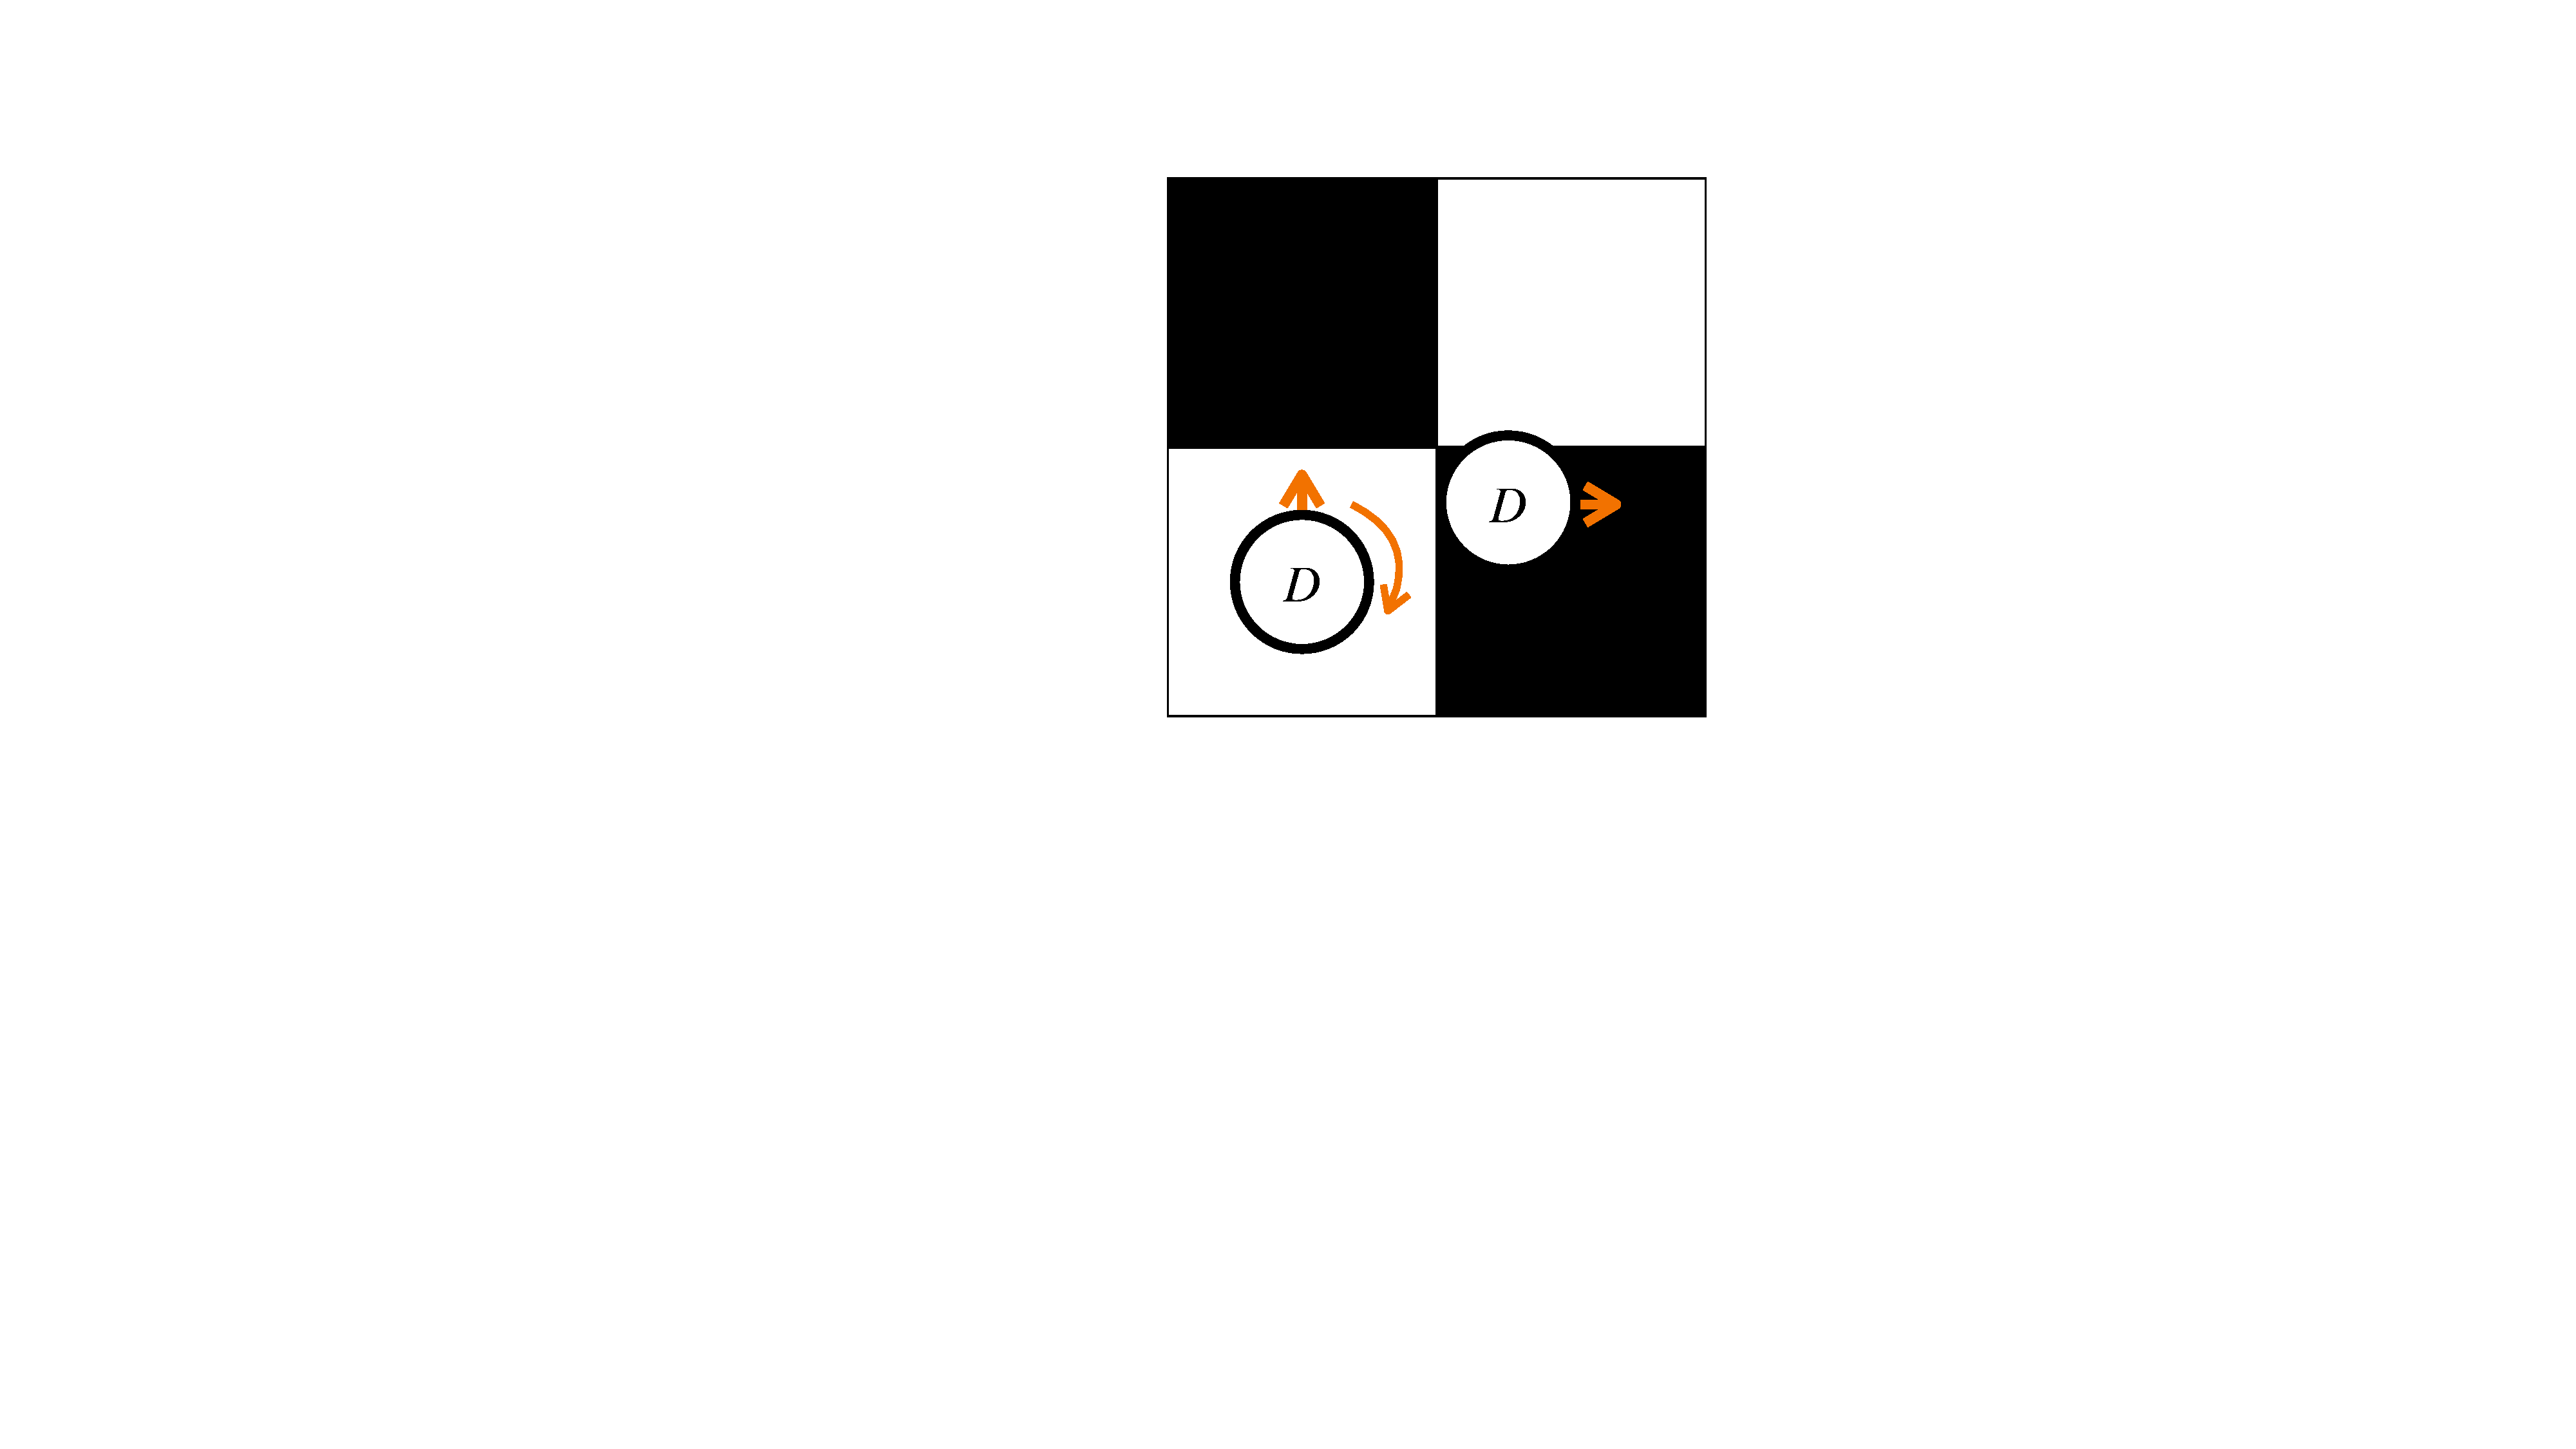
\includegraphics[width=0.4\textwidth]{../assets/dezibot_rotation_position_offset.pdf}
    \caption{90°"=Rechts"=Bewegung des Dezibots. Links ist Aus"-gangs-, rechts eine beispielhafte Endposition nach der Rotation abgebildet.}
    \label{fig:dezibot-rotation-position-offset}
\end{figure}


\subsection{Iteration 2: Allgemeine Move"=Funktion}
\label{sec:general-move-function}

Das Ziel der nächsten Iteration bestand darin, dem Dezibot nur ein Feld zu übergeben, auf das er sich bewegen soll. Diese Funktion wurde in der \texttt{ECP"-Chess"-Piece::""move(ECP"-Chess"-Field new"-Field)}"=Funktion implementiert. Sie bewegt den Dezibot vom aktuellen Feld zum übergebenen \texttt{new"-Field}.

Dabei wird zunächst mit der \texttt{is"-Move"-Valid}"=Funktion überprüft, ob der gewünschte Zug gültig ist (vgl. \autoref{sec:move-validation}). Die Gültigkeit wird vor einer Bewegung über die LEDs des Dezibots dargestellt. Falls der Zug gültig ist, wird dies durch grünes Licht angezeigt. Andernfalls zeigt der Dezibot rotes Licht und beendet vorzeitig durch die Rückgabe von \texttt{false}, ohne sich zu bewegen.

% Contraints: zurück rotieren

Dabei haben wir die folgenden Constraints aufgestellt: der Dezibot soll stets nach einem abgeschlossenen Zug in dieselbe Richtung schauen. Weiße Figuren schauen dabei stets in den Norden, schwarze in den Süden. Dies ist in orange in \autoref{fig:move-function-sketch} angedeutet.

\begin{figure}[h]
    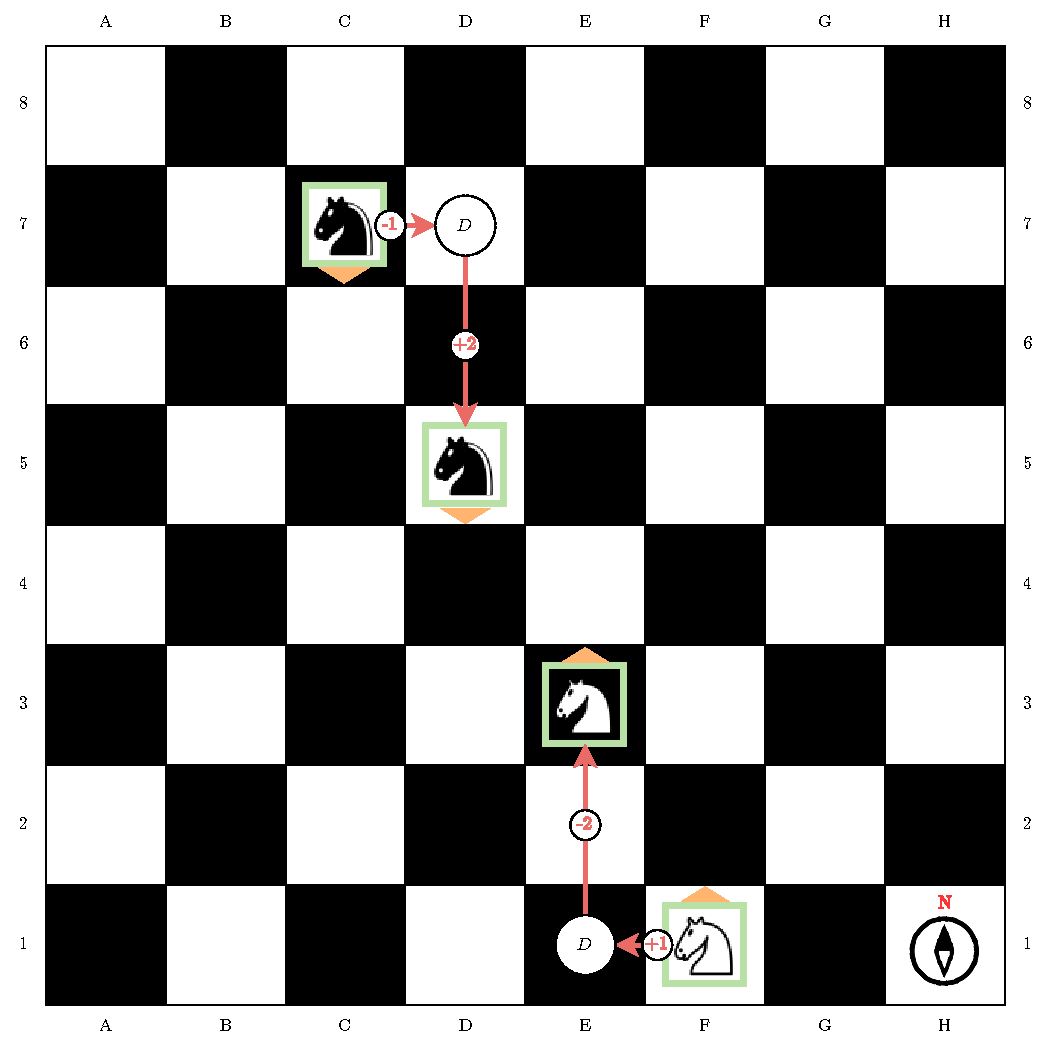
\includegraphics[width=\textwidth]{../assets/move_function_sketch.drawio.pdf}
    \caption{Veranschaulichung der Funktionalität von \texttt{move}. In orange ist die Ausrichtung des Dezibots, in rot die Differenz zwischen dem aktuellen und Zielfeld dargestellt.}
    \label{fig:move-function-sketch}
\end{figure}

% Zusammensetzung der Bewegung

Eine Bewegung setzt wie folgt zusammen: Zunächst bewegt sich der Dezibot horizontal in die korrekte Spalte und anschließend vertikal in die richtige Zeile. Dafür wird die Spalten"= bzw. Zeilen"=Differenz vom aktuellen Feld zum neuen Feld berechnet.

\begin{equation*}
    \begin{aligned}
        \Delta\text{col} &= \text{col}_{\text{current}} - \text{col}_{\text{new}} \\
        \Delta\text{row} &= \text{row}_{\text{current}} - \text{row}_{\text{new}}
    \end{aligned}
\end{equation*}

Anschließend wird die horizontale Bewegung ausgeführt, falls $\Delta\text{col} \ne 0$ gilt. Entsprechend des Vorzeichens wird die neue Richtung bestimmt, d.h. ob der Dezibot sich nach Osten oder Westen drehen muss. Basierend auf der aktuellen Richtung des Dezibots, welche in \texttt{ECP"-Chess"-Pieces::""current"-Direction} gespeichert ist, wird berechnet, in welche Richtung sich der Dezibot rotieren muss. Anschließend bewegt sich der Dezibot um $\vert \Delta\text{col} \vert$ Felder vorwärts.

Ähnlich funktioniert die vertikale Bewegung. Die basiert auf der Zeilen"=Differenz $\Delta\text{row}$ sowie der Nord"=Süd"=Achse. Erneut wird berechnet, wie rotiert werden muss. Danach folgt die Vorwärtsbewegung um $\vert \Delta\text{row} \vert$ Felder.

Nachdem der Dezibot auf dem korrekten Feld steht, dreht sich der Dezibot bei Bedarf zurück in die initiale Richtung. Somit drehen sich weiße Figuren wieder nach Norden; schwarze Figuren nach Süden. Dies beendet die Bewegung zum gewünschten Feld.

% Diskussion / Probleme

Insgesamt ergibt sich aus dem oben genannten Constraintsystem folgende Überlegungen. Es ergibt sich der Nachteil, dass sich Rotationsfehler, auf welche in \autoref{sec:plausibility-check-rotation} genauer eingegangen wird, addieren. Allerdings ist das Display nach einem abgeschlossenen Zug stets gleich zur spielenden Person ausgerichtet. Dadurch sieht das Schachbrett optisch einheitlich aus, da alle Figuren derselben Farbe in dieselbe Richtung schauen, wodurch die Optik mehr einem echten Schachbrett entspricht und die Übersichtlichkeit unterstützt. Weiterhin werden Display"=Ausgaben korrekt und nicht kopfüber dargestellt, wodurch diese einfacher durch die entsprechende spielende Person abzulesen sind. Ein weiterer Vorteil besteht darin, dass sich die Züge stets aus einer einheitlichen Bewegungs"= und Rotationsreihenfolge zusammensetzen, wodurch diese vorhersehbar ist. Somit überwiegen die Vorteile des Contraintsystems, besonders wenn die Probleme der Rotationsfehler behandelt werden.


\subsection{Iteration 3: Plausibilitätsprüfung der Rotation}
\label{sec:plausibility-check-rotation}

Wie bereits in \autoref{sec:move-straight-turn} erwähnt, ist die Rotation nach einer fest definierten Zeit aufgrund von unvorhersehbaren äußeren Einflüssen unzuverlässig und führt meist nicht zum gewünschten Ergebnis. Weiterhin rotiert der Dezibot nicht auf einem \enquote{Fleck}, sondern bewegt sich an eine andere, nicht deterministische Position. Dabei kann es passieren, dass der Dezibot, der ursprünglich auf einem weißen Feld stand, anschließend auf einem schwarzem steht (vgl. \autoref{fig:dezibot-rotation-position-offset}) oder vice versa. Daher wurde eine Plausibilitätsprüfung für die Rotation als Verbesserung eingeführt, welche überprüft, ob die Farbe des initialen Feldes dieselbe ist, wie die jenes Feldes, welches nach einer Rotation erreicht wurde.

Bei einer Rotation wird zunächst mit der in \autoref{sec:move-straight-turn} erwähnten \texttt{ECP"-Color"-Detection::""is"-White"-Field}"=Funktion gemessen, ob der Dezibot ursprünglich auf einem weißen oder schwarzem Feld steht. Nach einer Rotation wird dies erneut gemessen und mit dem ursprünglichen Wert verglichen. Wenn die Farben übereinstimmen, wird die Rotation als plausibel gewertet. Andernfalls wird eine Nachricht auf dem Display des Dezibots angezeigt, welche eine manuelle Korrektur anfordert. Dabei wird das gewünschte Feld sowie die Richtung, nach der der Dezibot ausgerichtet werden soll, ausgegeben. Eine Beispiel"=Ausgabe ist in \autoref{fig:display-rotation-correction-request} dargestellt.

\begin{figure}[h]
\centering
\begin{cminted}{text}
+----------------+
|Faulty rotation |
|Please correct  |
|my position     |
|within 10s to   |
|                |
|> A1 NORTH      |
|                |
|Thank you!      |
+----------------+
\end{cminted}
\caption{Beispiel für Aufforderung zur Korrektur einer fehlgeschlagenen Rotation. Gewünscht ist Feld \texttt{A1} mit Ausrichtung \texttt{NORTH}.}
\label{fig:display-rotation-correction-request}
\end{figure}

Somit können fehlerhafte Rotationen, welche den Dezibot unerwünscht auf ein anderes Feld bewegen, von den Spielenden korrigiert werden. Starke Abweichungen, d.h. Rotation auf ein anderes Feld derselben Farbe, können dabei jedoch nicht erkannt werden. Dies ist jedoch selten der Fall.

Mit dieser Verbesserung kann ebenfalls nicht überprüft werden, ob eine intendierte 90°"=Drehung den Dezibot auch tatsächlich um 90° dreht. Dieses Problem wurde in der folgenden Iteration thematisiert.


\subsection{Iteration 4: Infrarot"=basierte Rotation}
\label{sec:movement-ir}

Zur Verbesserung der Rotation wogen wir einige Ideen ab. Einerseits bauten wir bereits die im vorherigen Abschnitt erläuterte Plausibilitätsprüfung der Rotation ein. Eine zusätzliche Idee war es, ein Regelsystem für die Rotation zu entwerfen und zu implementieren. Die Farbe bzw. das Licht vom Untergrund wird bereits die Plausibilitätsprüfung betrachtet. Insgesamt war der Wunsch, eine zweite physikalisch Größen einzubeziehen.

Der Beschleunigungssensor (\emph{Inertial Measurement Unit}, IMU) entfiel dabei als mögliche Option, da dieser aktuell nur im Ansatz von der existierenden \texttt{dezibot}"=Library unterstützt wird und viel Low"=Level"=Code notwendig wäre. Während den Lehrveranstaltungen wurde jedoch von große Problemen mit der Genauigkeit beschrieben. Daher wurde sich für den folgenden, anderen Ansatz entschieden.

Diese basiert auf einer zusätzlichen Signalquelle (\emph{Beacon}), aus welcher die relative Ausrichtung des Dezibots trigonometrisch approximiert werden kann. Vorstellbar sind hier WLAN- oder Bluetooth"=Signale, oder auch Infrarot"=Licht. Schlussendlich entschieden wir uns durch die Abwägung von Kosten und Nutzen für die Infrarot"=LED eines Dezibots als Beacon sowie die seitlichen "=Sensoren zur Messung. Diese sind in \autoref{fig:dezibot-bottom} hervorgehoben.

\begin{figure}[h]
    \centering
    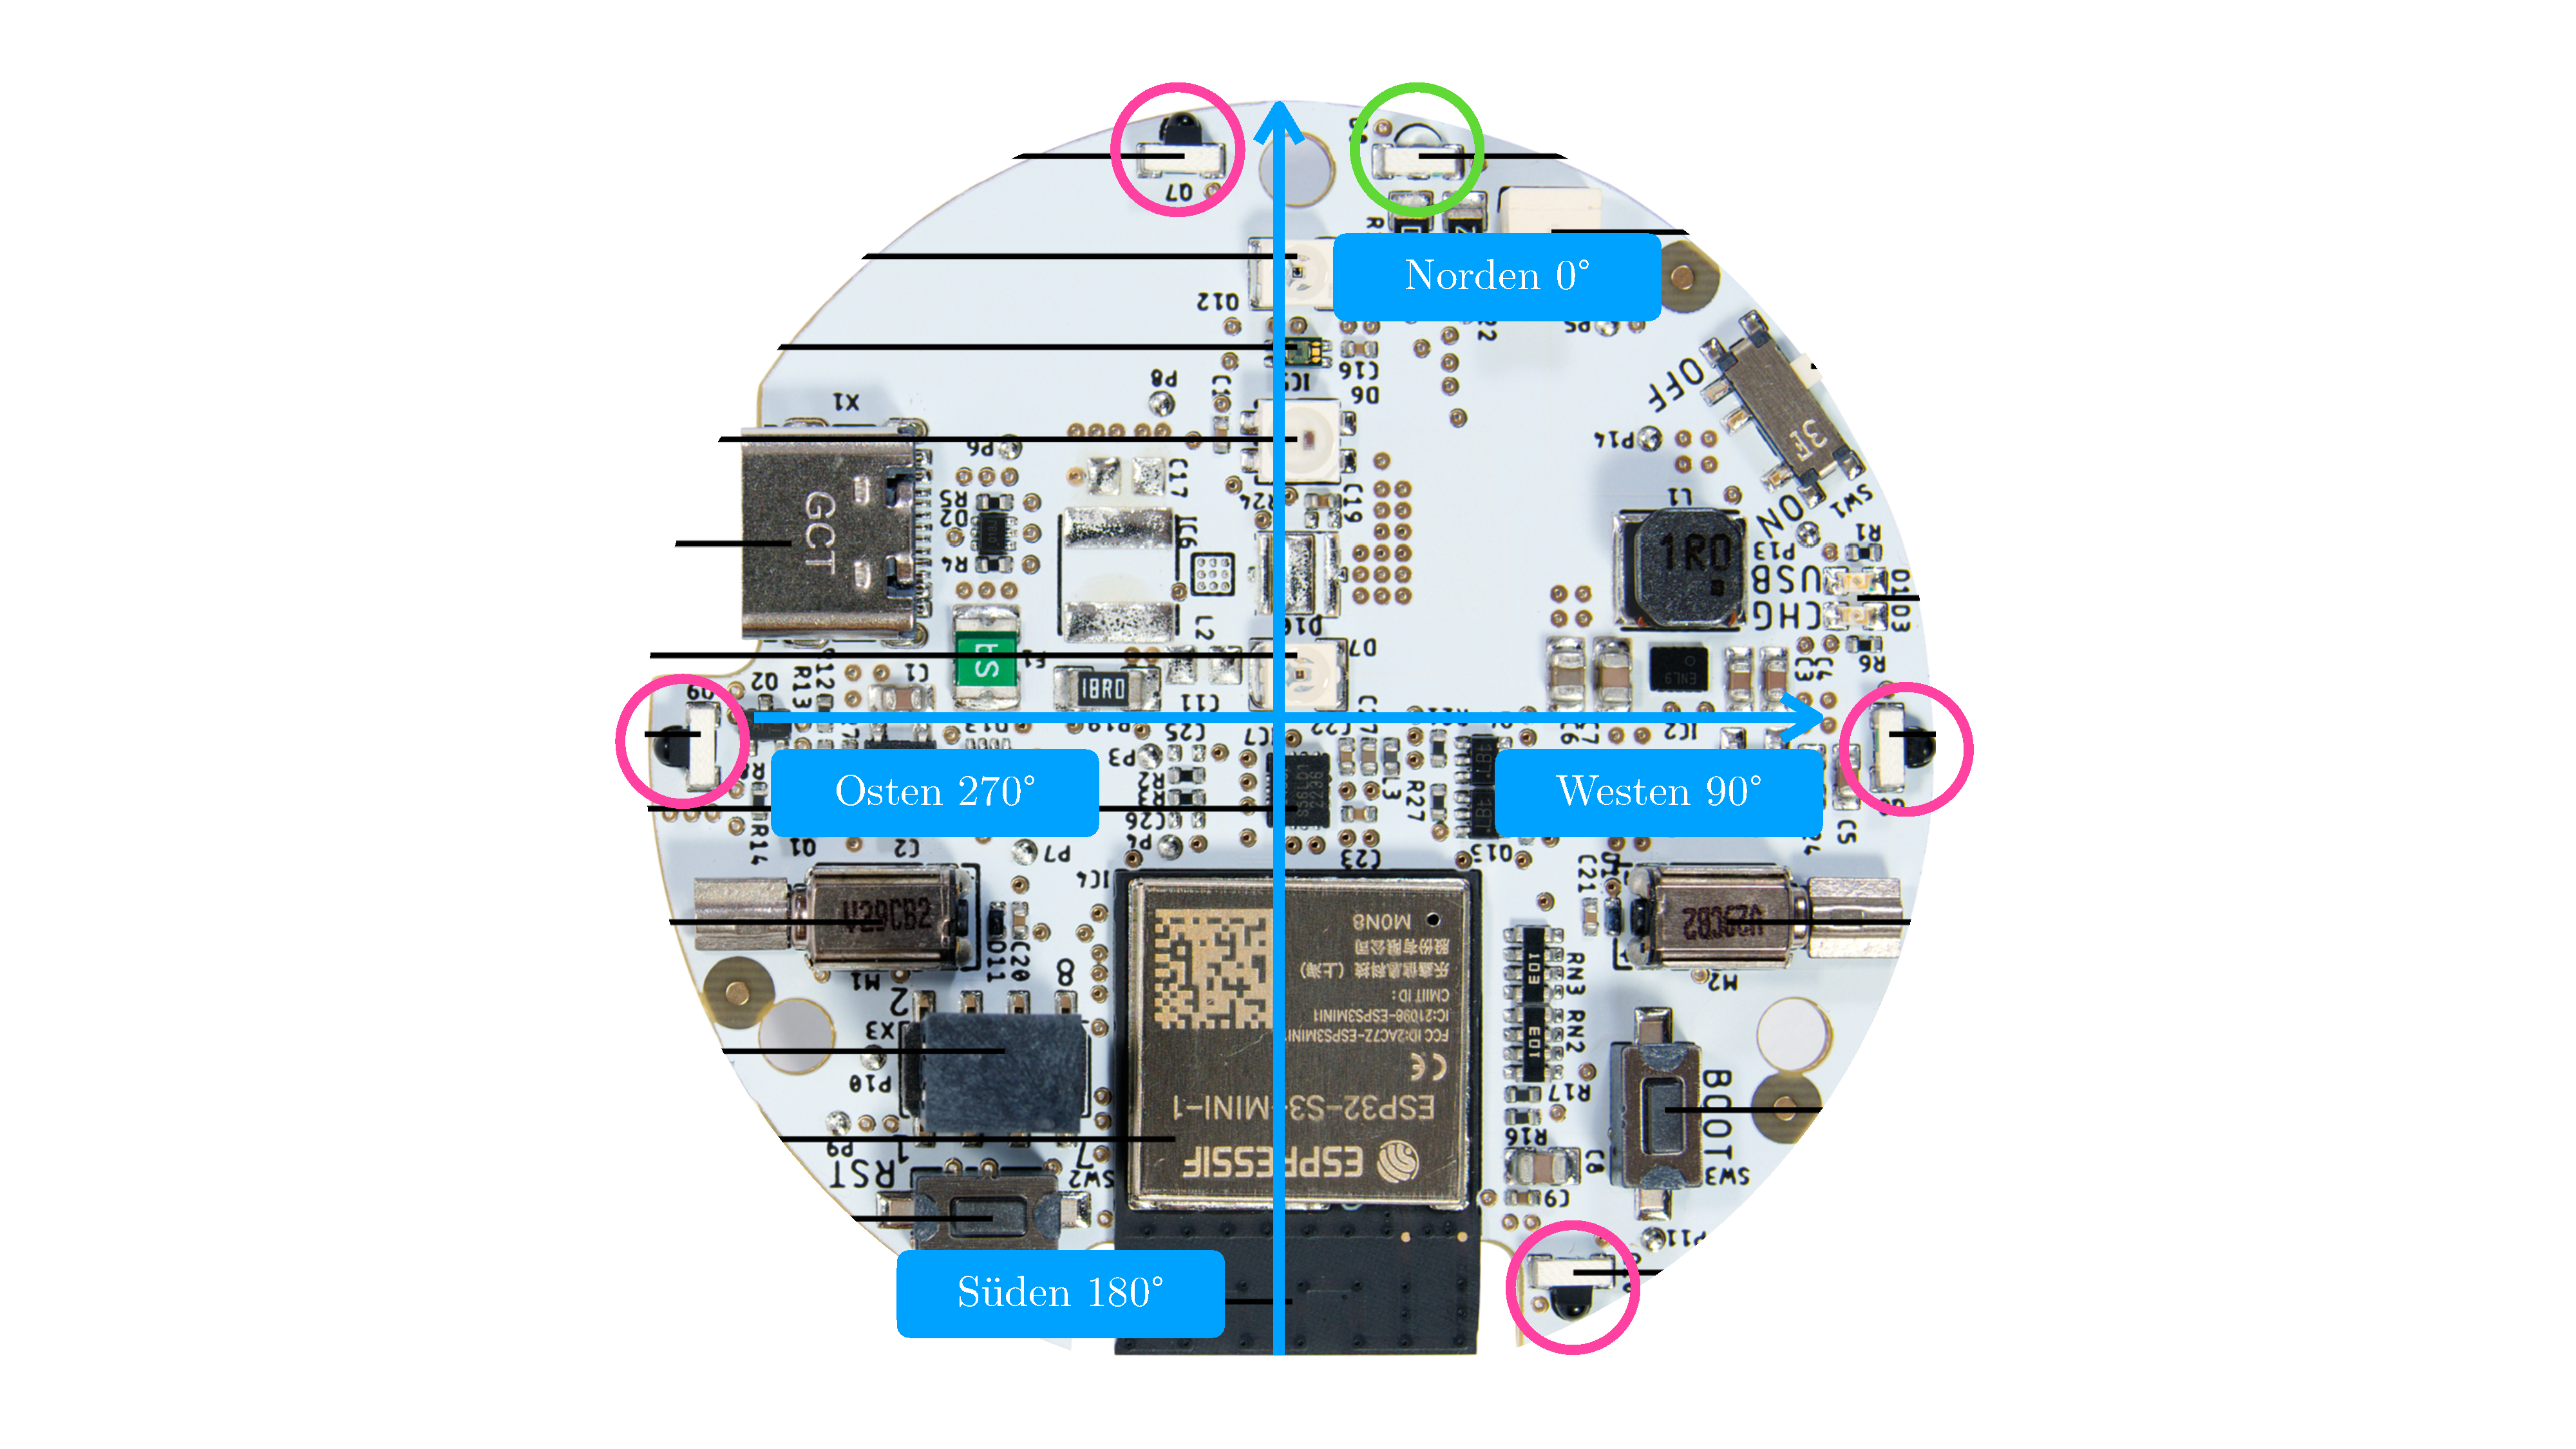
\includegraphics[width=0.8\textwidth]{../assets/dezibot_bottom.pdf}
    \caption{Unterseite des Dezibots, auf der die verwendete Infrarot"=LED in grün sowie die seitlichen Infrarot"=Sensoren in magenta umrandet sind. In blau sind die Himmelsrichtungen mit den entsprechenden (relativen) Winkel der Dezibot"=Ausrichtung eingezeichnet. West und Ost sind hier gespiegelt, da es sich hierbei um die Unterseite des Dezibots handelt. Grafik wurde aus~\cite{fingerleDokumentationDezibot42025} entnommen, bearbeitet und annotiert.}
    \label{fig:dezibot-bottom}
\end{figure}

Dafür wird ein Dezibot, welcher ein Infrarot"=Signal aussendet, neben dem Schachbrett platziert, welches ungefähr in die Mitte des Schachbretts schaut. Dafür wurde das Programm {\texttt{ir\_emitter.ino} geschrieben, welches ebenjene Funktion erfüllt.

Dieses Signal wird von \texttt{ECP"-Signal"-Detection::""measure"-Signal"-Angle} gemessen. Dabei werden der Werte von allen vier Infrarot"=Sensoren gelesen und verrechnet. Aus dem gemessenen Winkel des Beacon"=Signals wird der Winkel berechnet, in den der Dezibot in Relation zum Beacon ausgerichtet ist (vgl. \texttt{ECPSignal"-Detection::""measure"-Dezi"-bot"-Angle}). Die beiden Winkel sind in \autoref{fig:signal-dezibot-angle} verdeutlicht. Die Bestimmung der Winkel wird in \autoref{sec:angle-determination} genauer erläutert.

\begin{figure}[h]
    \centering
    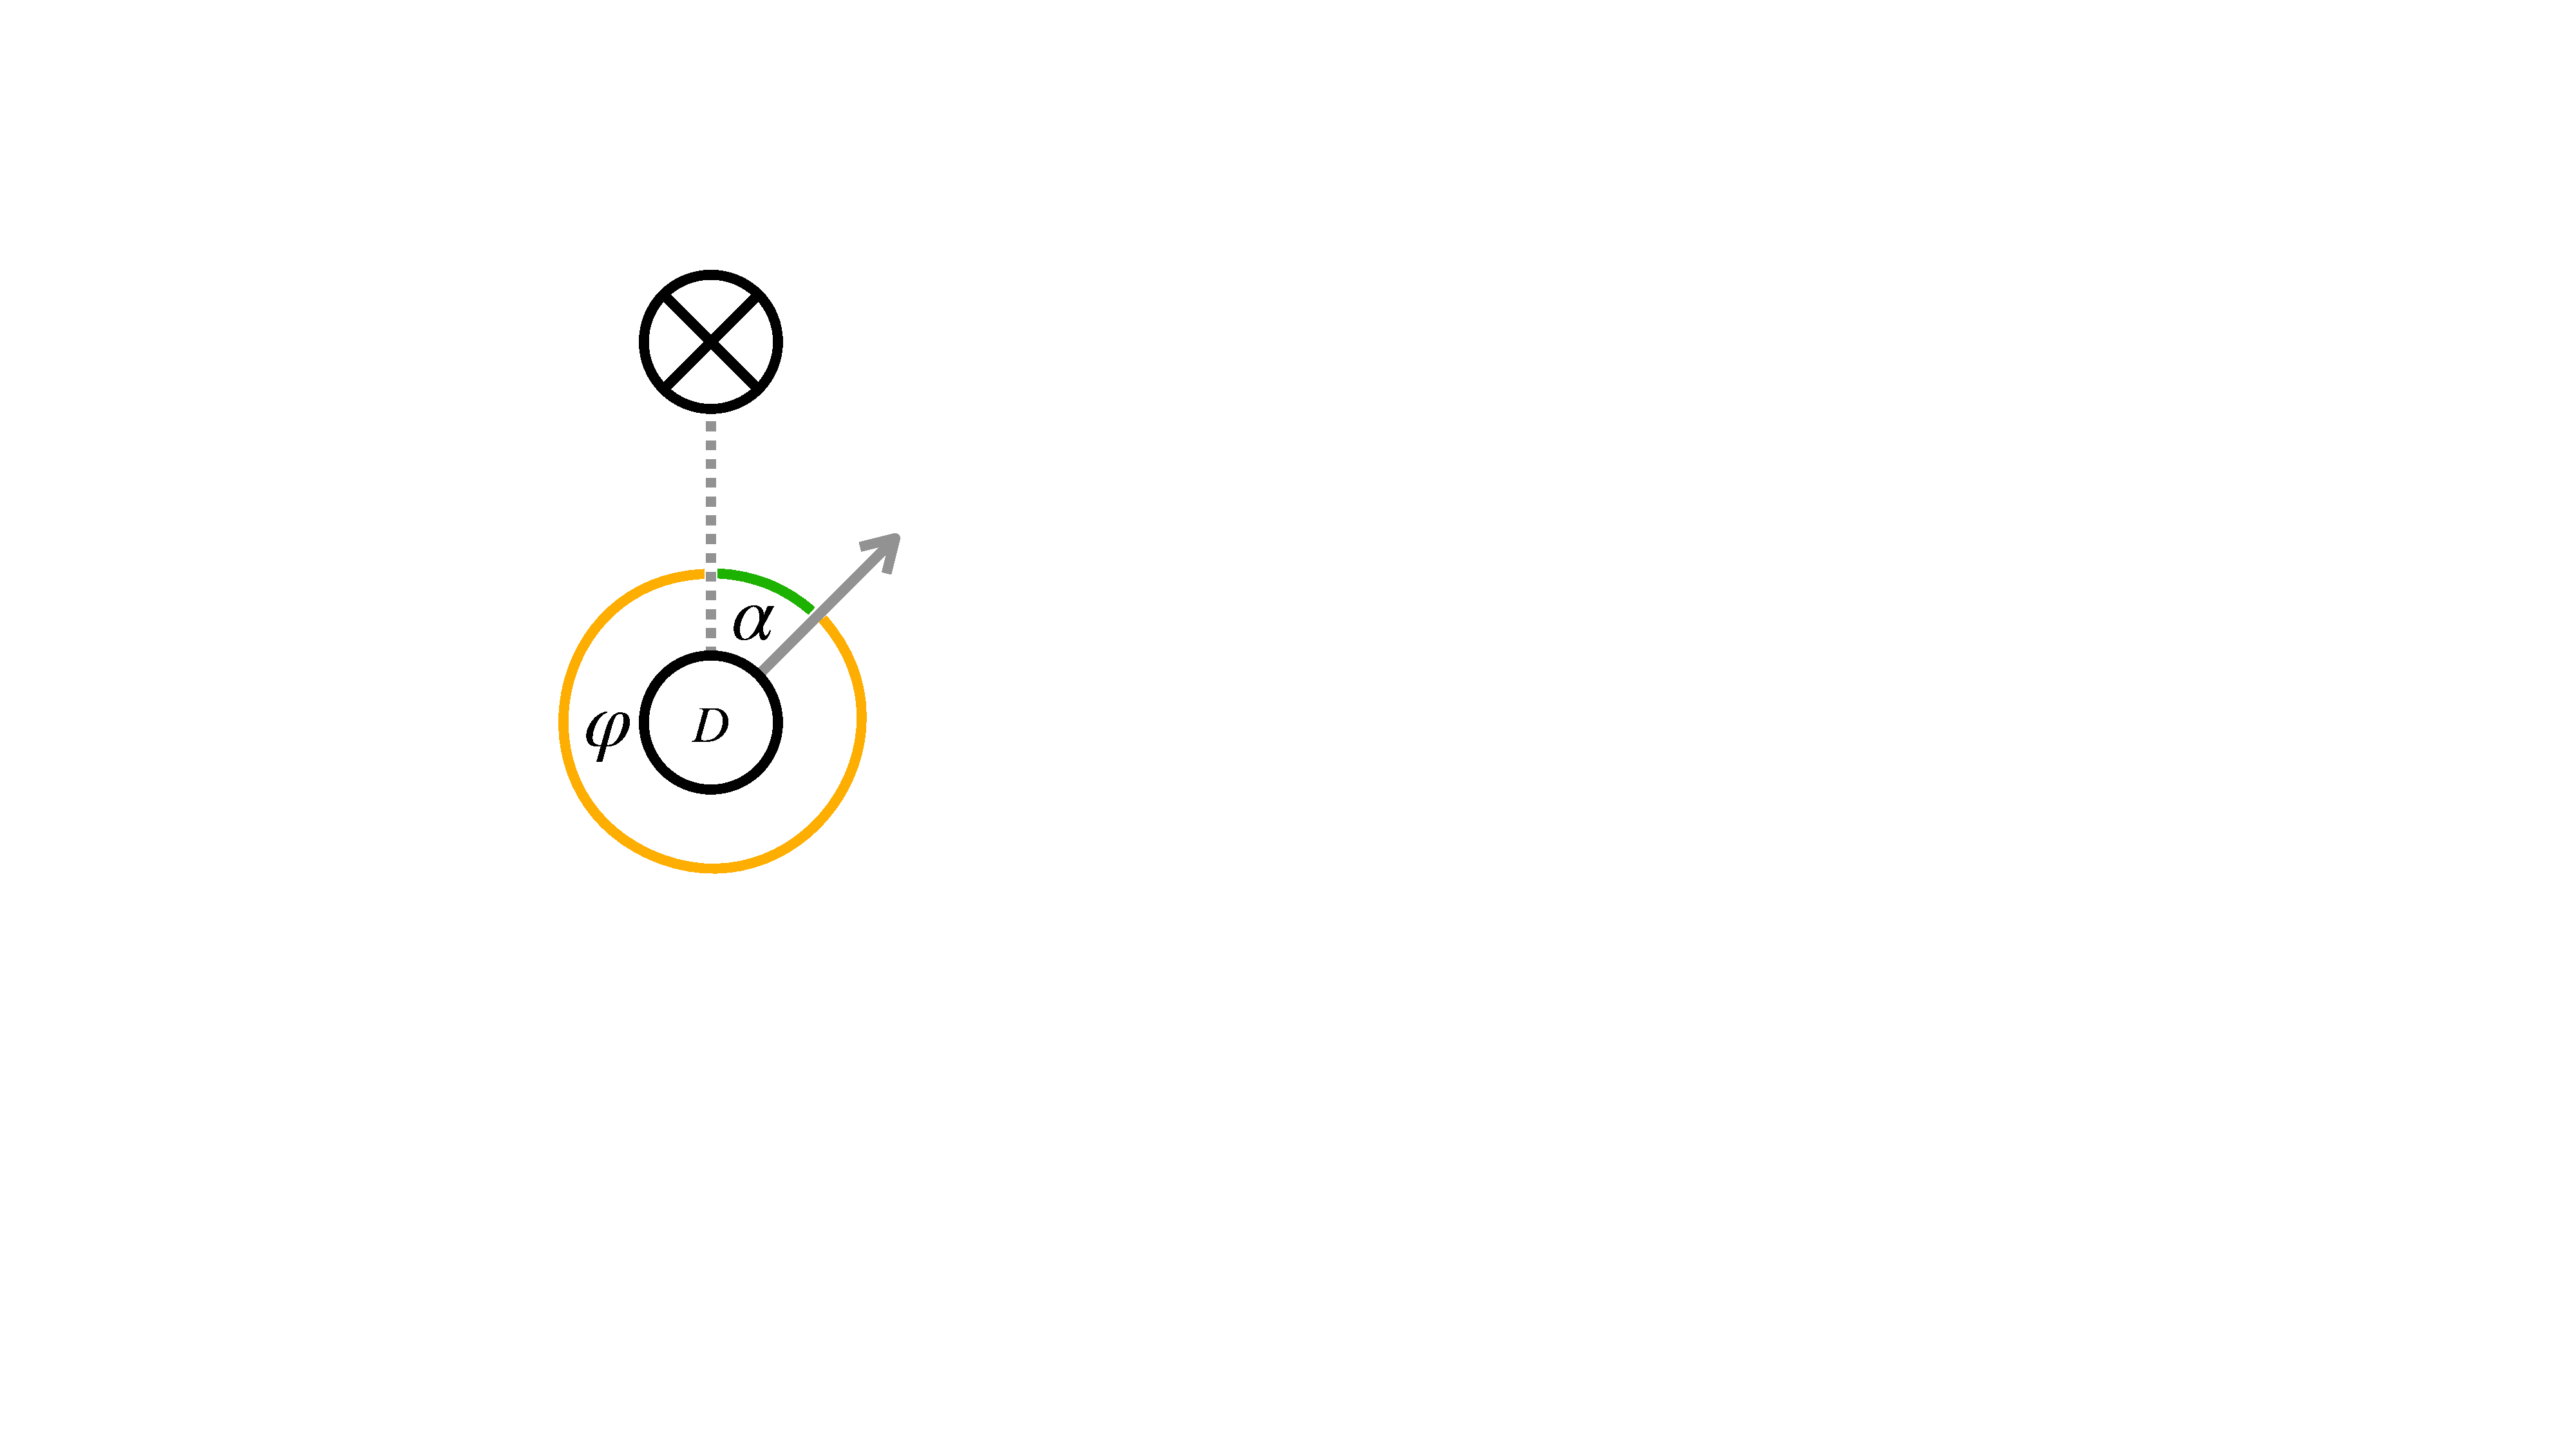
\includegraphics[width=0.2\textwidth]{../assets/signal_dezibot_angle.pdf}
    \caption{Skizze zur Darstellung des gemessenen Signal"=Winkels $\varphi$ vom Beacon sowie des dazu relativen Dezibot"=Aus"-rich"-tungs"-winkels~$\alpha$. $D$~markiert den messenden Dezibot, $\otimes$~den Beacon. Der von $D$ ausgehende graue Pfeil, zeigt die Ausrichtung des Dezibots an.}
    \label{fig:signal-dezibot-angle}
\end{figure}

Nachdem der Winkel berechnet wurde, wird ein Ziel"=Winkel~$\alpha'$ berechnet. Wenn sich der Dezibot nach links drehen soll, werden 90° vom initialen Winkel~$\alpha$ subtrahiert, bei einer Rotation nach rechts 90° addiert. Damit der Winkel bei einer Links"=Rotation nicht negativ wird, werden zunächst 360° addiert. Anschließend wird auf den Wert der Modulo 360 angewendet. Insgesamt folgt ein Ziel"=Winkel~$\alpha' \in [0,360] \subset \mathbb{N}$.

\begin{equation*}
\begin{aligned}
    \text{Rotation links } &\implies \alpha' = (\alpha - 90\degree + 360\degree) \operatorname{mod} 360\degree \\
    \text{Rotation rechts } &\implies \alpha' = (\alpha + 90\degree) \operatorname{mod} 360\degree
\end{aligned}
\end{equation*}

An diesem Punkt sind die zwei wichtigen Größen bekannt: einerseits der initiale Winkel~$\alpha$, in dem der Dezibot relativ zum Beacon \emph{vor} der Rotation steht; andererseits der relative Ziel"=Winkel~$\alpha'$, in dem der Dezibot nach der Rotation ausgerichtet sein soll. Eine Skizze ist in \autoref{fig:dezibot-rotation-angles} abgebildet.

\begin{figure}[h]
    \centering
    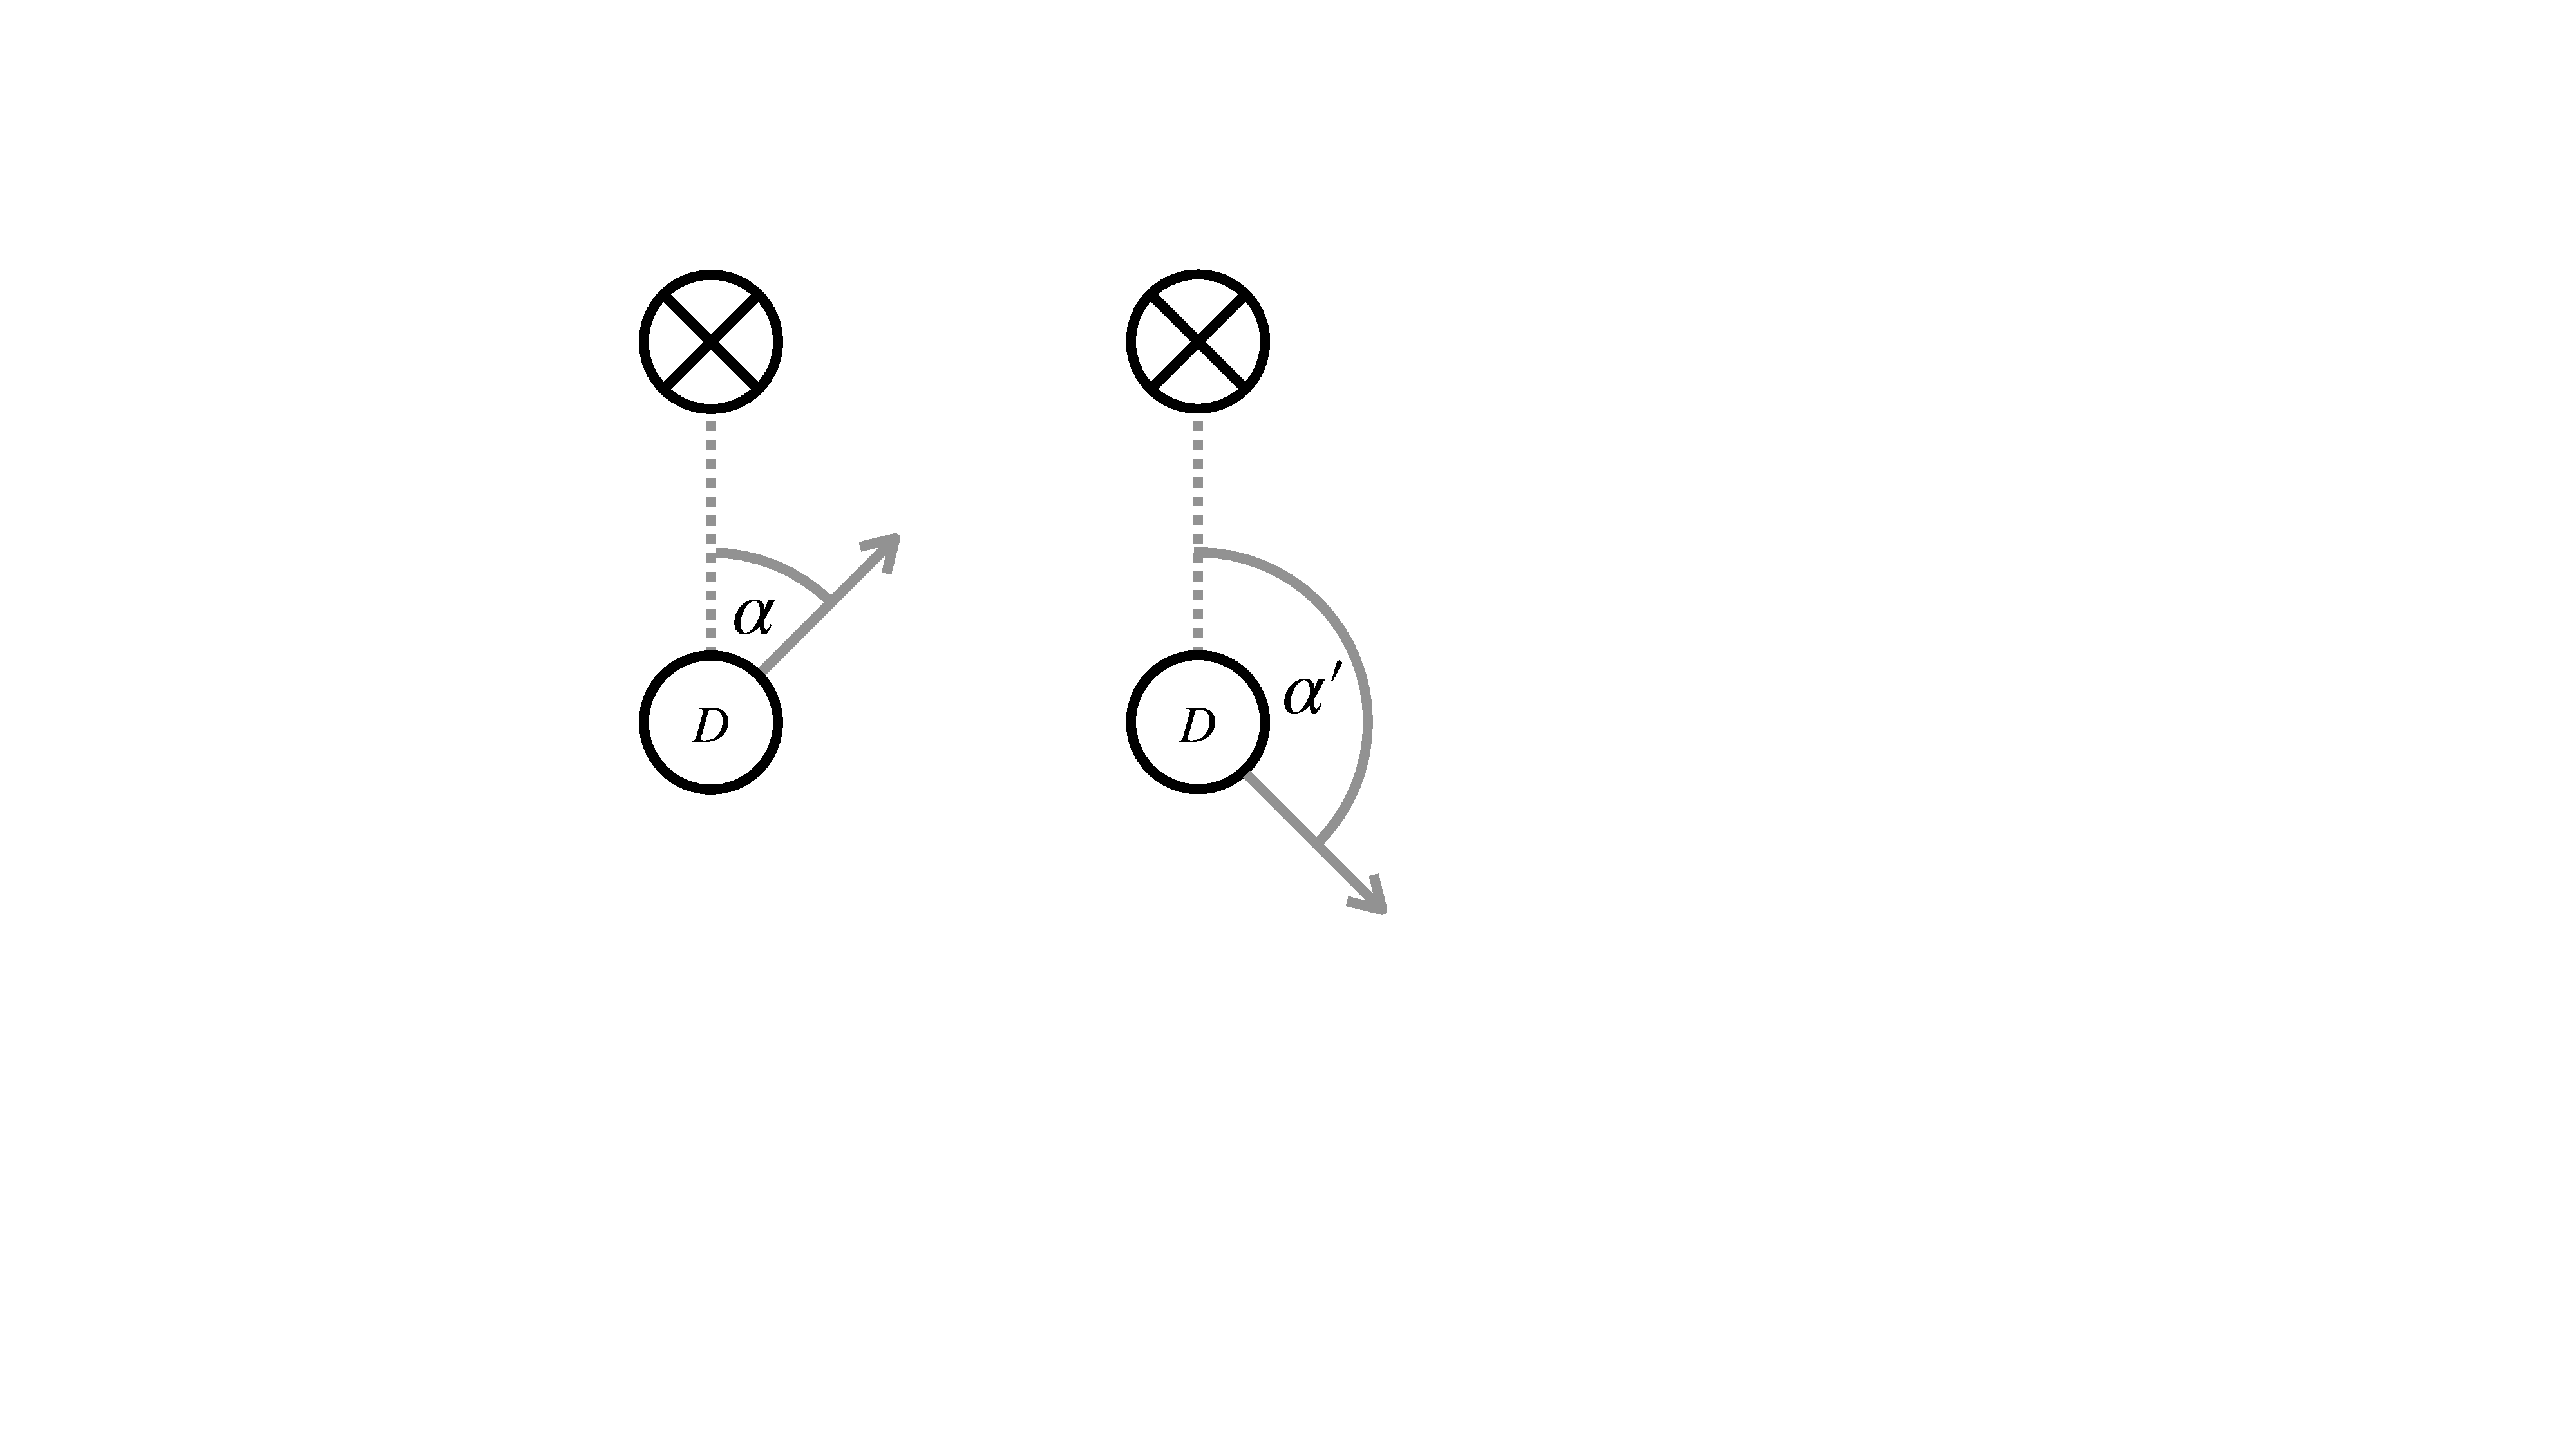
\includegraphics[width=0.5\textwidth]{../assets/dezibot_rotation_angles.pdf}
    \caption{Rotation des Dezibots vom initialen Winkel $\alpha$ (linke Seite) zum Ziel"=Winkel $\alpha'$ (rechte Seite). $D$~markiert den rotierenden Dezibot, $\otimes$~den Beacon. Der von $D$~ausgehende graue Pfeil, zeigt die Ausrichtung des Dezibots an.}
    \label{fig:dezibot-rotation-angles}
\end{figure}

Mit diesen beiden Werten wird die \texttt{ECPMove"-ment"-::"-rotate"-To"-Angle}"=Funktion aufgerufen. Diese rotiert den Dezibot inkrementell vom übergebenen initialen Winkel zum Ziel"=Winkel. Dabei wird innerhalb einer Schleife basierend auf der normalisierten Differenz $\Delta\theta_{\text{norm}}$ bestimmt, ob der Dezibot am effizientesten nach links oder rechts rotieren muss, um $\alpha'$ zu erreichen. Dies wird in \autoref{sec:rotation-direction-determination} genauer erläutert. Anschließend wird die benötigte Rotationszeit approximiert.

Die Approximation basiert auf Experimenten aus \autoref{sec:move-straight-turn}, welche ergeben haben, dass eine Rotation um 180° etwa 5 Sekunden benötigt. Basierend auf der absoluten normalisiert Differenz $\vert\Delta\theta_{\text{norm}}\vert$ wird der folgende angenommene Approximation verwendet:

\begin{equation*}
    180\degree \cdot 28~\frac{\text{ms}}{\degree} = 5040~\text{ms} \approx 5000~\text{ms}
\end{equation*}

Dementsprechend ergibt sich die approximierte Rotationszeit $t_{\text{r}}$ wie folgt:

\begin{equation*}
    t_{\text{r}} \approx \vert\Delta\theta{\text{norm}}\vert \cdot 28~\frac{\text{ms}}{\degree}
\end{equation*}

Dementsprechend wird die approximierte Rotationszeit geringer, je kleiner die normalisierte Differenz wird. Das heißt, je näher sich der Dezibot am gewünschten Ziel"=Winkel $\alpha'$ ausgerichtet ist, desto kürzer wird rotiert. Anschließend wird der Dezibot, je nach kürzester Rotationsrichtung, in die entsprechende Richtung für $t_{\text{r}}$ rotiert.

Nach dem Rotationsinkrement wird der neue relative Winkel des Dezibots erneut gemessen, d.h. $\alpha$ aktualisiert, und das Verfahren von vorn durchgeführt. Die Rotationsrichtung und "=zeit werden erneut berechnet, wodurch ein Gegensteuern möglich ist, falls sich der Dezibot zu weit bewegt hat. Eine Rotation wird außerdem als erfolgreich bewertet, wenn der neue Winkel $\alpha$ innerhalb einer festgelegten Toleranz -- aktuell 3° -- befindet. Diese Toleranz ist in der Konstante \texttt{ECPMove"-ment::""ROTA"-TION\_TOLER"-ANCE} definiert.

Falls innerhalb von 20 Iterationen der Ziel"=Winkel nicht erreicht werden konnte, wird analog zu \autoref{sec:plausibility-check-rotation} eine Aufforderung zur manuellen Korrektur durch die Spielenden aufgefordert.


\subsubsection{Bestimmung der Winkel}
\label{sec:angle-determination}

In diesem Abschnitt wird die Bestimmung des Winkels $\varphi$, in dem das Infrarot"=Signal beim Dezibot eintrifft, sowie wie der Dezibot in Relation dazu ausgerichtet ist $\alpha$ bestimmt wird. Diese Funktionalitäten entsprechen den Funktionen \texttt{measure"-Signal"-Angle} sowie \texttt{measure"-Dezi"-bot"-Angle} aus der Klasse \texttt{ECPSig"-nal"-Detec"-tion}. Die Winkel sind in \autoref{fig:signal-dezibot-angle} skizziert.
 
Zunächst werden die vier Werte der seitlichen Infrarot"=Sensoren gelesen. Dabei werden jeweils drei Messungen mit einem Abstand von jeweils 30 Millisekunden gemittelt, um die Ergebnisse zu verbessern. Die Ergebnisse liegen auf einer Skala von $[0,4095]$ vor, welche zunächst auf $[0,1] \subset \mathbb{R}$ normalisiert werden, um eine leichtere Weiterverarbeitung zu ermöglichen. Anschließend wird überprüft, ob mindestens ein Messwert über einem festgelegten Schwellwert (0.1, d.h. 10~Prozent) liegt, um eine gewisse Signalstärke vorauszusetzen. Falls dies nicht der Fall ist, wird eine entsprechende Warnung auf das Display gedruckt. Nach einer Sekunde wird erneut versucht, einen gültigen Wert zu lesen. Dies geschieht solange, bis ein signifikanter Wert gemessen werden kann.

Nachdem hinreichende Signalmessungen vorliegen, kann der Winkel Beacon"=Signals berechnet werden. Dazu werden die Nord"=Süd"= $r_{y}$ sowie Ost"=West"=Resultanten $r_{x}$ des Ergebnisvektors $R$ berechnet. Dabei sind $n,s,e$ und $w$ jeweils die Signalmessungen aus Nord"=, Süd"=, Ost"= bzw. West"=Richtung.

\begin{equation*}
    r_{x} = e - w, \quad r_{y} = n - s, \quad R = (r_x~r_y)^T
\end{equation*}

Aus den Resultanten wird der Winkel $\varphi$ vom Ergebnisvektor $R$ berechnet.

\begin{equation*}
    \varphi = \arctan_2(r_{x}, r_{y}) \cdot \frac{180\degree}{\pi}
\end{equation*}

Eine Veranschaulichung der Resultanten, des Ergebnisvektors sowie des Winkels~$\varphi$ sind anhand von Beispiel"=Daten in \autoref{fig:angle-determination-beacon} abgebildet.

\begin{figure}[h]
    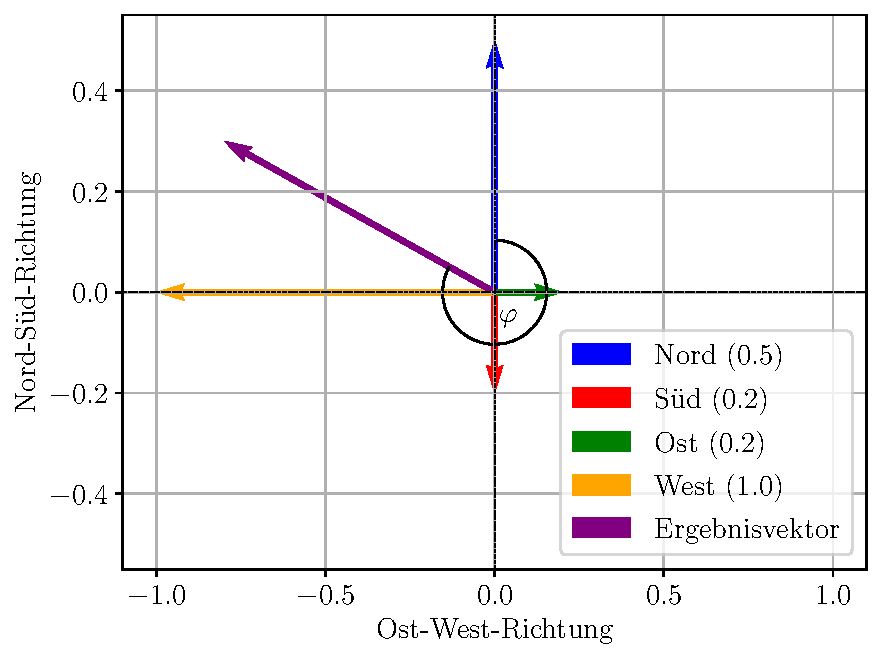
\includegraphics[width=\textwidth]{../plot/signal_direction.pdf}
    \caption{Veranschaulichung der Berechnung des Signal"=Winkels~$\varphi$ anhand eines Beispiels; Messwerte siehe Legende. Grafik wurde mittels \href{https://matplotlib.org/}{Matplotlib} unter Verwendung von~\cite{matplotlibdevelopmentteamScaleInvariantAngle} erstellt.}
    \label{fig:angle-determination-beacon}
\end{figure}

Anschließend wird in \texttt{ECPSignal"-Detec"-tion::""measure"-Dezi"-bot"-Angle} der Winkel~$\alpha$ bestimmt, in den der Dezibot relativ zum Beacon ausgerichtet ist (vgl.~\autoref{fig:signal-dezibot-angle}).

\vspace{-1em}
\begin{equation*}
    \alpha = (360\degree - \varphi) \operatorname{mod} 360\degree
\end{equation*}


\subsubsection{Bestimmung der Rotationsrichtung}
\label{sec:rotation-direction-determination}

Im folgenden Abschnitt wird erläutert, wie der kürzeste Weg, um den gewünschten Ziel"=Winkel~$\alpha'$ vom initialen Dezibot"=Winkel $\alpha$ zu erreichen, errechnet wird -- das heißt, ob es effizienter ist, den Dezibot nach links oder rechts zu rotieren. Dafür wird zunächst die Differenz beider Winkel~$\Delta\theta$ gebildet und normiert zu~$\Delta\theta_{\text{norm}}$.

\vspace{-1em}
\begin{equation*}
\begin{aligned}
    \Delta\theta &= \alpha' - \alpha \\
    \Delta\theta_{\text{norm}} &= \big( (\Delta\theta + 180\degree) \operatorname{mod} 360\degree \big) - 180\degree
\end{aligned}
\end{equation*}

Basierend auf $\Delta\theta_{\text{norm}}$ kann wie folgt entschieden werden, in welche Richtung am effizientesten rotiert werden muss:

\vspace{-1em}
\begin{equation*}
\begin{aligned}
    \Delta\theta_{\text{norm}} < 0\degree &\Rightarrow \text{Links-Rotation} ~(\circlearrowleft)\\
    \Delta\theta_{\text{norm}} > 0\degree &\Rightarrow \text{Rechts-Rotation} ~(\circlearrowright)\\
    \Delta\theta_{\text{norm}} \in \lbrace 0\degree, 180\degree \rbrace &\Rightarrow \text{egal} \leadsto \text{Links-Rotation} ~(\circlearrowleft)
\end{aligned}
\end{equation*}

Diese Gedanken werden in \texttt{ECPMove"-ment::""rotate"-To"-Angle} umgesetzt.


\subsubsection{Auftretende Probleme}

Insgesamt ist die Infrarot"=basierte Rotation der aktuell vielversprechenste Versuch, der zur Abgabe der Arbeit implementiert ist.
% TODO: Prüfen vor Abgabe!
Dennoch sind einige Probleme aufgetreten, die im folgenden erläutert werden.

% Problem: Unterschiede in IR-Sensoren

Es ist problematisch, wenn die Messungen je nach Infrarot"=Sensor (herstellungsbedingt) abweichen. Dies kann beispielsweise durch äußere Einflüsse, wie Beschmutzungen der Sensoren, entstehen. Außerdem sind die Nord"= und Süd"=Sensoren (vgl. \autoref{fig:dezibot-bottom}) neben einem Bein platziert, wodurch das Blickfeld verkleinert wird und ggf. Schatten (vgl. \autoref{fig:dezibt-ir-shadow}) und somit blinde Flecken sowie ggf. Reflexionen entstehen. Ungenauigkeiten, die bei der Herstellung entstehen, können ggf. weitere Messungenauigkeiten verursachen.

\begin{figure}[h]
    \centering
    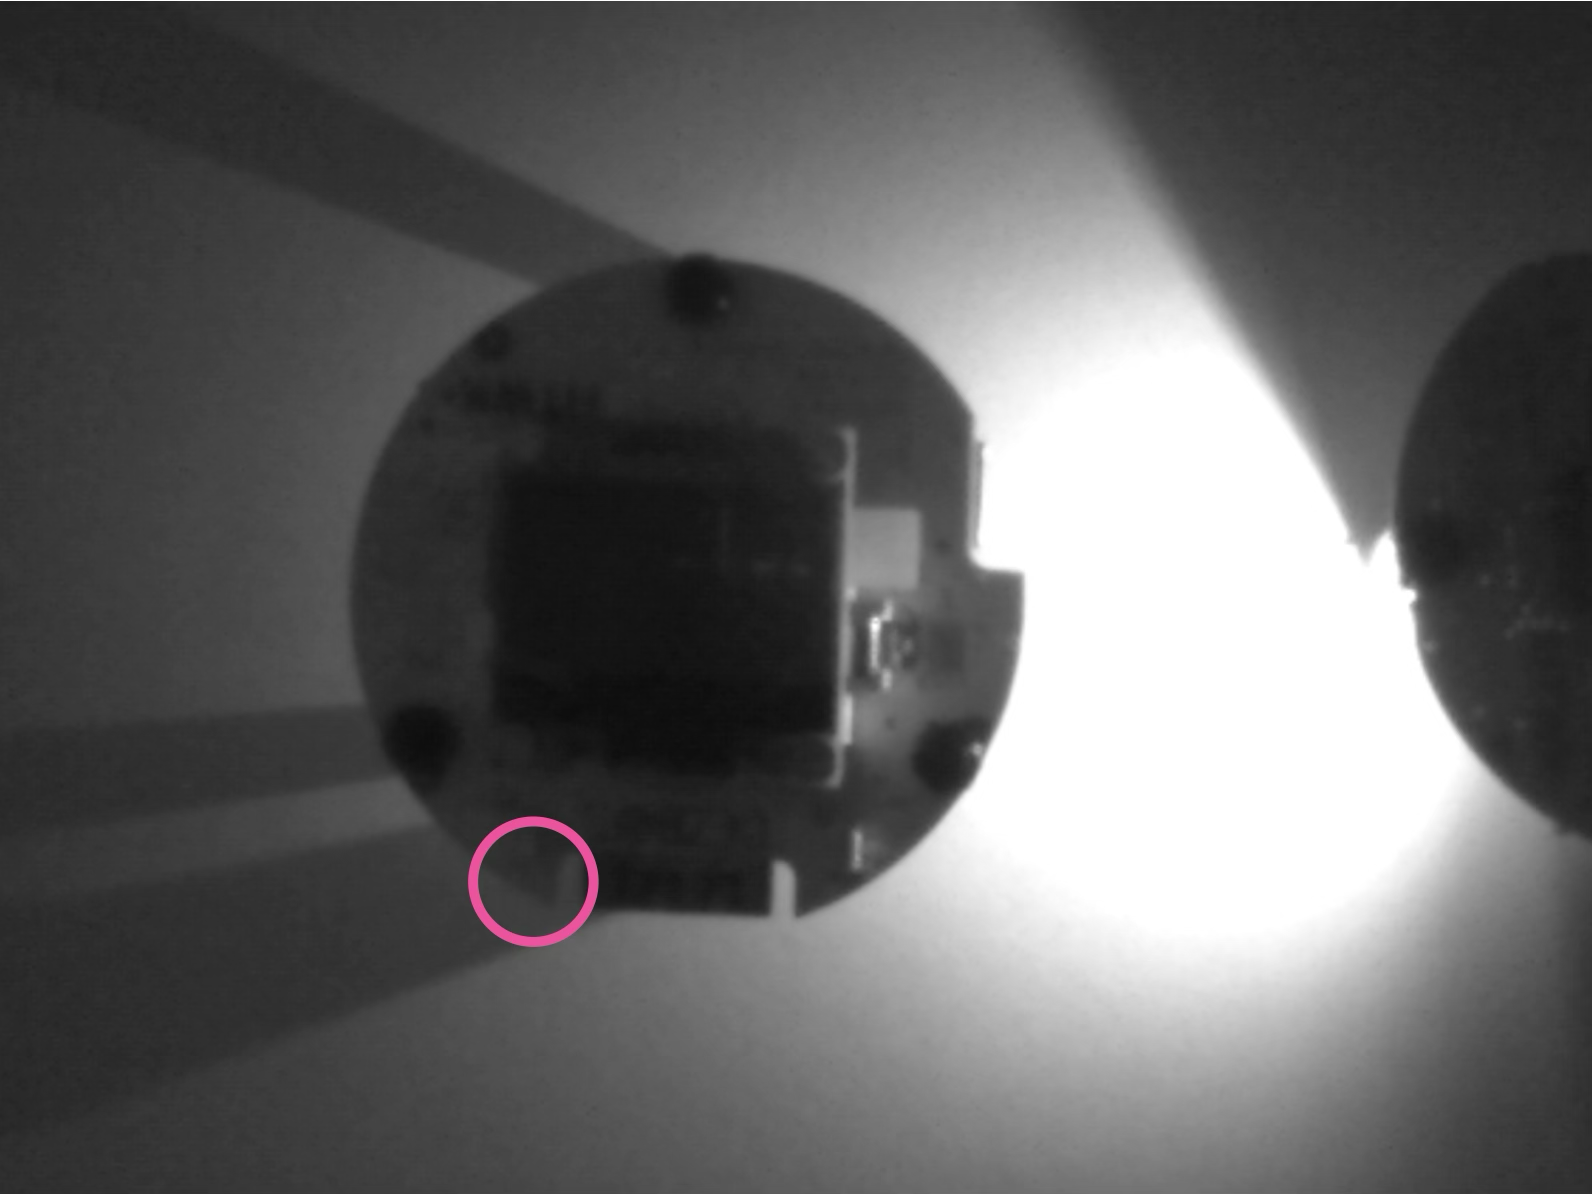
\includegraphics[width=0.8\textwidth]{../assets/dezibot_ir_shadow.png}
    \caption{Schatten, welche durch die Beine des Dezibots entstehen. Rechts ist ein Beacon"=Dezibot abgeschnitten zu sehen. Der südliche Infrarot"=Sensor ist in magenta hervorgehoben. (Infrarot"=Aufnahme)}
    \label{fig:dezibt-ir-shadow}
\end{figure}

% Problem: IR-Sensoren nicht auf 90° platziert, off-axis

Weiterhin ist in \autoref{fig:dezibot-bottom} zu erkennen, dass die magenta umrandeten Infrarot"=Sensoren nicht exakt auf der (virtuellen) $x$"= bzw. $y$"=Achse platziert sind. Daher ist die Berechnung des Signal"=Winkels (vgl. \autoref{sec:angle-determination}) nicht exakt, da dort davon ausgegangen wird, dass diese exakt auf der jeweiligen Achse in gleichem Abstand zum Mittelpunkt des Dezibots (virtueller Koordinatenursprung) liegen. Da dies allerdings nicht der Fall ist, ist die Berechnung ungenau. Je nach Ursprungsrichtung des Infrarot"=Signales weicht die Differenz bei einigen Richtungen des Dezibots unterschiedlich stark ab. Weiterhin behindern die Beine des Dezibots die Messungen, da diese das Sichtfeld beeinträchtigen.

Dazu wurden zwei kleine, begrenzte Messstudien durchgeführt, die diese Tatsache verdeutlichen. Ein Beacon wurde dafür im Norden bzw. 0° bezüglich des messenden Dezibots positioniert. In der ersten Studie wurden die Ergebnisse der Signal"=Messungen von \texttt{ECP"-Signal"-Detection::""measure"-Dezibot"-Angle} in verschiedenen Winkeln gemessen. Die Ergebnisse sind in \autoref{tab:measurements-dezibot-angle} in \autoref{sec:measurements-dezibot-angle} dargestellt. Die Differenzen der Messungen zu den eigentlichen Signal"=Winkeln in in \autoref{fig:ir-signal-diff} dargestellt.

\begin{figure}[h]
    \centering
    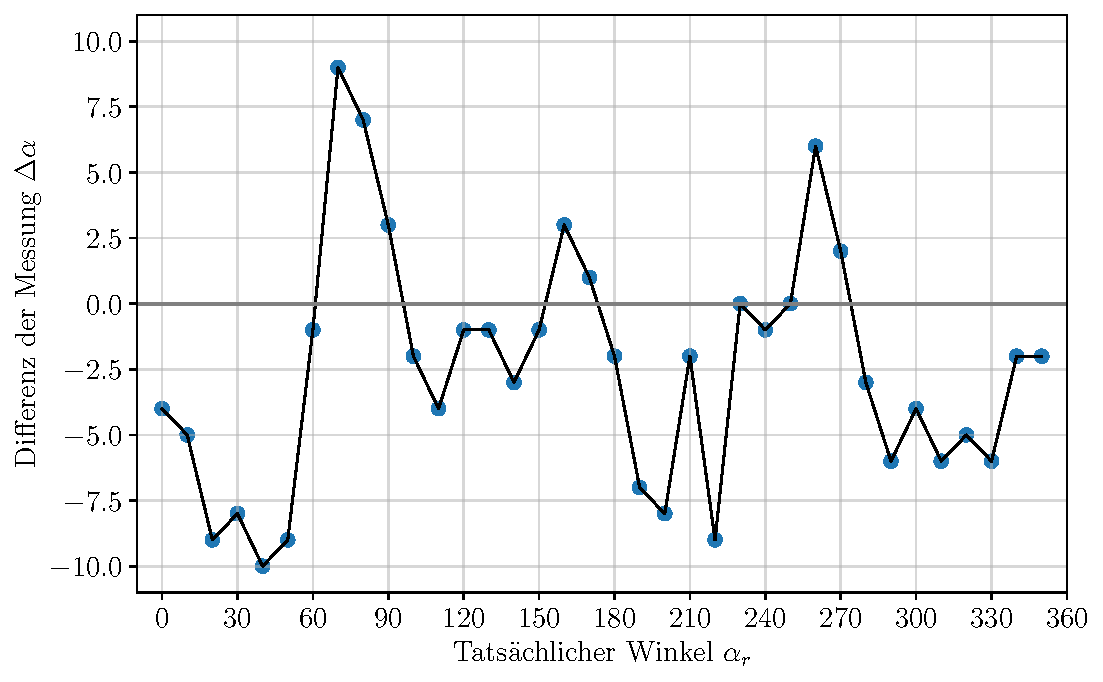
\includegraphics[width=\textwidth]{../plot/ir_signal_diff.pdf}
    \caption{Diagramm der Differenz der Signal"=Messungen bezüglich des tatsächlichen Winkels. Daten basieren auf \autoref{tab:measurements-dezibot-angle}.}
    \label{fig:ir-signal-diff}
\end{figure}

In der zweiten Messstudie wurde eine Infrarot"=basierte Links"= bzw. Rechts"=Rotation vom Dezibot durchgeführt. Dabei wurde der Dezibot in die vier verschiedenen Himmelsrichtungen ausgerichtet. Insgesamt wurden jeweils fünf Versuche durchgeführt. Die Messwerte sind in \autoref{tab:measurements-dezibot-angle} in \autoref{sec:measurements-ir-rotation} aufgelistet. Die daraus resultierenden durchschnittlichen Differenzen zwischen dem Ziel"= und dem tatsächlich erreichten Winkel sowie die Standardabweichungen der Messungen pro Rotationsart sind in \autoref{tab:measurements-dezibot-angle-avg-dev} dargestellt.

\begin{table}[h]
    \centering
    \begin{tabular}{c|c|c|c}
    & Rotation & $\varnothing$ Differenz & Standardabweichung \\ \hline\hline
    %
    \multirow{4}{*}{L} & 0° $\to$ 270°   & 9,2°   & 1,10° \\
                       & 90° $\to$ 0°    & -9,0°  & 2,65° \\
                       & 180° $\to$ 90°  & 1,0°   & 1,73° \\
                       & 270° $\to$ 180° & 0,0°   & 2,00° \\ \hline\hline
    %
    \multirow{4}{*}{R} & 0° $\to$ 90°    & 15,2°  & 3,27° \\
                       & 90° $\to$ 180°  & 2,4°   & 2,88° \\
                       & 180° $\to$ 270° & 7,6°   & 2,51° \\
                       & 270° $\to$ 0°   & -10,4° & 0,89°
\end{tabular}

    \caption{Durchschnittliche Differenzen vom Ziel"= und dem tatsächlich erreichten Winkel sowie Standardabweichungen der Messungen pro Rotationsart von Links"= (L) und Rechts"=Rotationen (R) basierend auf den Daten aus \autoref{tab:measurements-dezibot-angle}.}
    \label{tab:measurements-dezibot-angle-avg-dev}
\end{table}

Aus \autoref{fig:ir-signal-diff} sowie \autoref{tab:measurements-dezibot-angle} wird erkenntlich, dass die Messungen sowie Rotationen sehr unregelmäßig schwanken. In \autoref{sec:ir-rotation-improvements} wird auf einige weitere Versuche zur Verbesserung eingegangen.

% Problem: andere IR-Quellen

Ein anderes Problem stellen zusätzliche Infrarot"=Quellen dar, wie beispielsweise die Sonne oder beliebige Reflexionen. Diese verschieben die Messungen, da die Berechnung des Beacon"=Winkels $\varphi$ auf den Vektoren der Nord"=Süd"= und Ost"=West"=Resultanten basiert. Wenn beispielsweise das Beacon"=Signal aus dem Norden kommt und die Sonne aus dem Süden strahlt, wird die Messung entsprechend nach Süden verschoben. So ist es denkbar, dass die Sonne den Beacon sogar vollständig überstrahlt, da die Sonne eine viel stärkere Infrarot"=Quelle ist, als das Beacon.

Zur Lösung wäre eine initiale Kalibrierung der Infrarot"=Messung denkbar. Falls die fremd"=einwirkenden, ungewünschten Infrarot"=Signale jedoch zu stark sind und die des Beacons überstrahlen, hilft dieser Ansatz nicht weiter. Daher ist eine Abdunkelung der Umgebung effektiver, um diesem Problem vollständig entgegenzuwirken.

Denkbar wäre jedoch eine Anpassung des Signals, welches vom Beacon ausgesendet wird, um von Störquellen unterscheiden zu können. So wäre eine Modulation, beispielsweise mittels \emph{On"=Off"=Keying} (Amplitudenumtastung, OOK), möglich. Dabei wird das ausgesendete Signal in bestimmten Intervallen ein"= und ausgeschaltet. 

Beim Empfang müssen die anderen Frequenzen herausgefiltert werden, zum Beispiel mittels Bandpassfilter. Damit ist eine Unterscheidung zwischen konstanten Störquelle und Beacon möglich. Dieses Prinzip wird u.a. bei handelsüblichen Fernbedienungen verwendet~\cite{ewaldIRFernbedienungen2019} und ist stark vereinfacht in \autoref{fig:on-off-keying} abgebildet.

\begin{figure}[h]
    \centering
    \begin{subfigure}{0.8\textwidth}
        \centering
        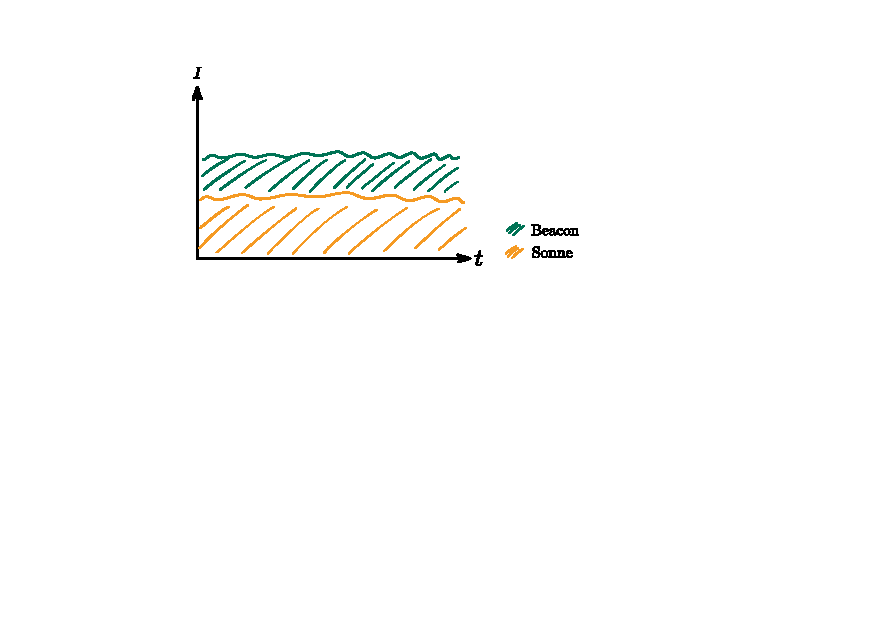
\includegraphics[width=\textwidth]{../assets/on-off-keying-1.pdf}
        \caption{Signalstärken ohne On"=Off"=Keying}
    \end{subfigure}
    \hspace{0.5cm}
    \begin{subfigure}{0.8\textwidth}
        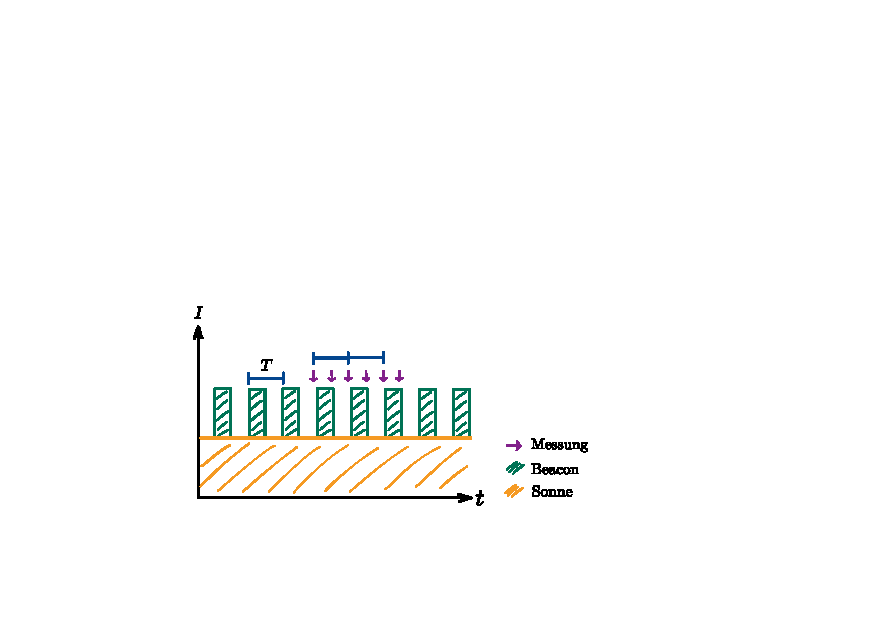
\includegraphics[width=\textwidth]{../assets/on-off-keying-2.pdf}
        \caption{Signalstärken mit On"=Off"=Keying (grün)}
    \end{subfigure}
    \caption{Diagramme der Signalstärke von Infrarot"=Signalen $I$ über die Zeit $t$ mit und ohne On"=Off"=Keying"=Prinzip zur Unterscheidung von Beacon und Sonne als exemplarische Störquelle (stark vereinfacht und nicht proportional)}
    \label{fig:on-off-keying}
\end{figure}

Da der Dezibot über keinen (Hardware"=) Bandpassfilter verfügt und die Berechnung in Software zu ressourcenintensiv wäre, muss ein optimierter Algorithmus entworfen werden. Dieser muss eine effiziente Filterung ermöglichen, um die Signale in Echtzeit zu unterscheiden.

Weiterhin wäre es möglich, dieses Problem zu lösen, in dem keine Infrarot"= sondern anderweitige, nicht natürlich vorkommende Signale verwendet werden, wie beispielsweise WLAN oder Bluetooth.

Mit dem Bluetooth 5.1 Standard wurde die \emph{Angle of Arrival} (AOA) Methode hinzugefügt. Damit ist es möglich, den Winkel bzw. die Richtung eines empfangenen Bluetooth"=Paketes zu approximieren~\cite[][Abschnitt 8.1]{bluetoothsigincBluetoothCoreSpecification2019}. Dies wäre sehr gut geeignet, um den Winkel des Beacons zu bestimmen, anstelle vom in \autoref{sec:angle-determination} erläuterten Algorithmus. Im Dezibot ist der ESP32-S3-MINI-1 verbaut~\cite{fingerleDokumentationDezibot42025}, welcher diese Methode jedoch (noch) nicht unterstützt~\cite{espressifsystemsshanghaico.ltdMajorFeatureSupport2024}.

Ein weiteres Problem besteht darin, dass sich der Dezibot bei der Rotation vom ursprünglichen Platz wegbewegt, da dieser sich nicht still um die eigene Achse drehen kann. Somit verändert sich der Beacon"=Winkel, selbst wenn der Dezibot sich nicht rotiert hat. Dieses Problem ist in \autoref{fig:dezibot_signal_moving_problem} veranschaulicht.

\begin{figure}[h]
    \centering
    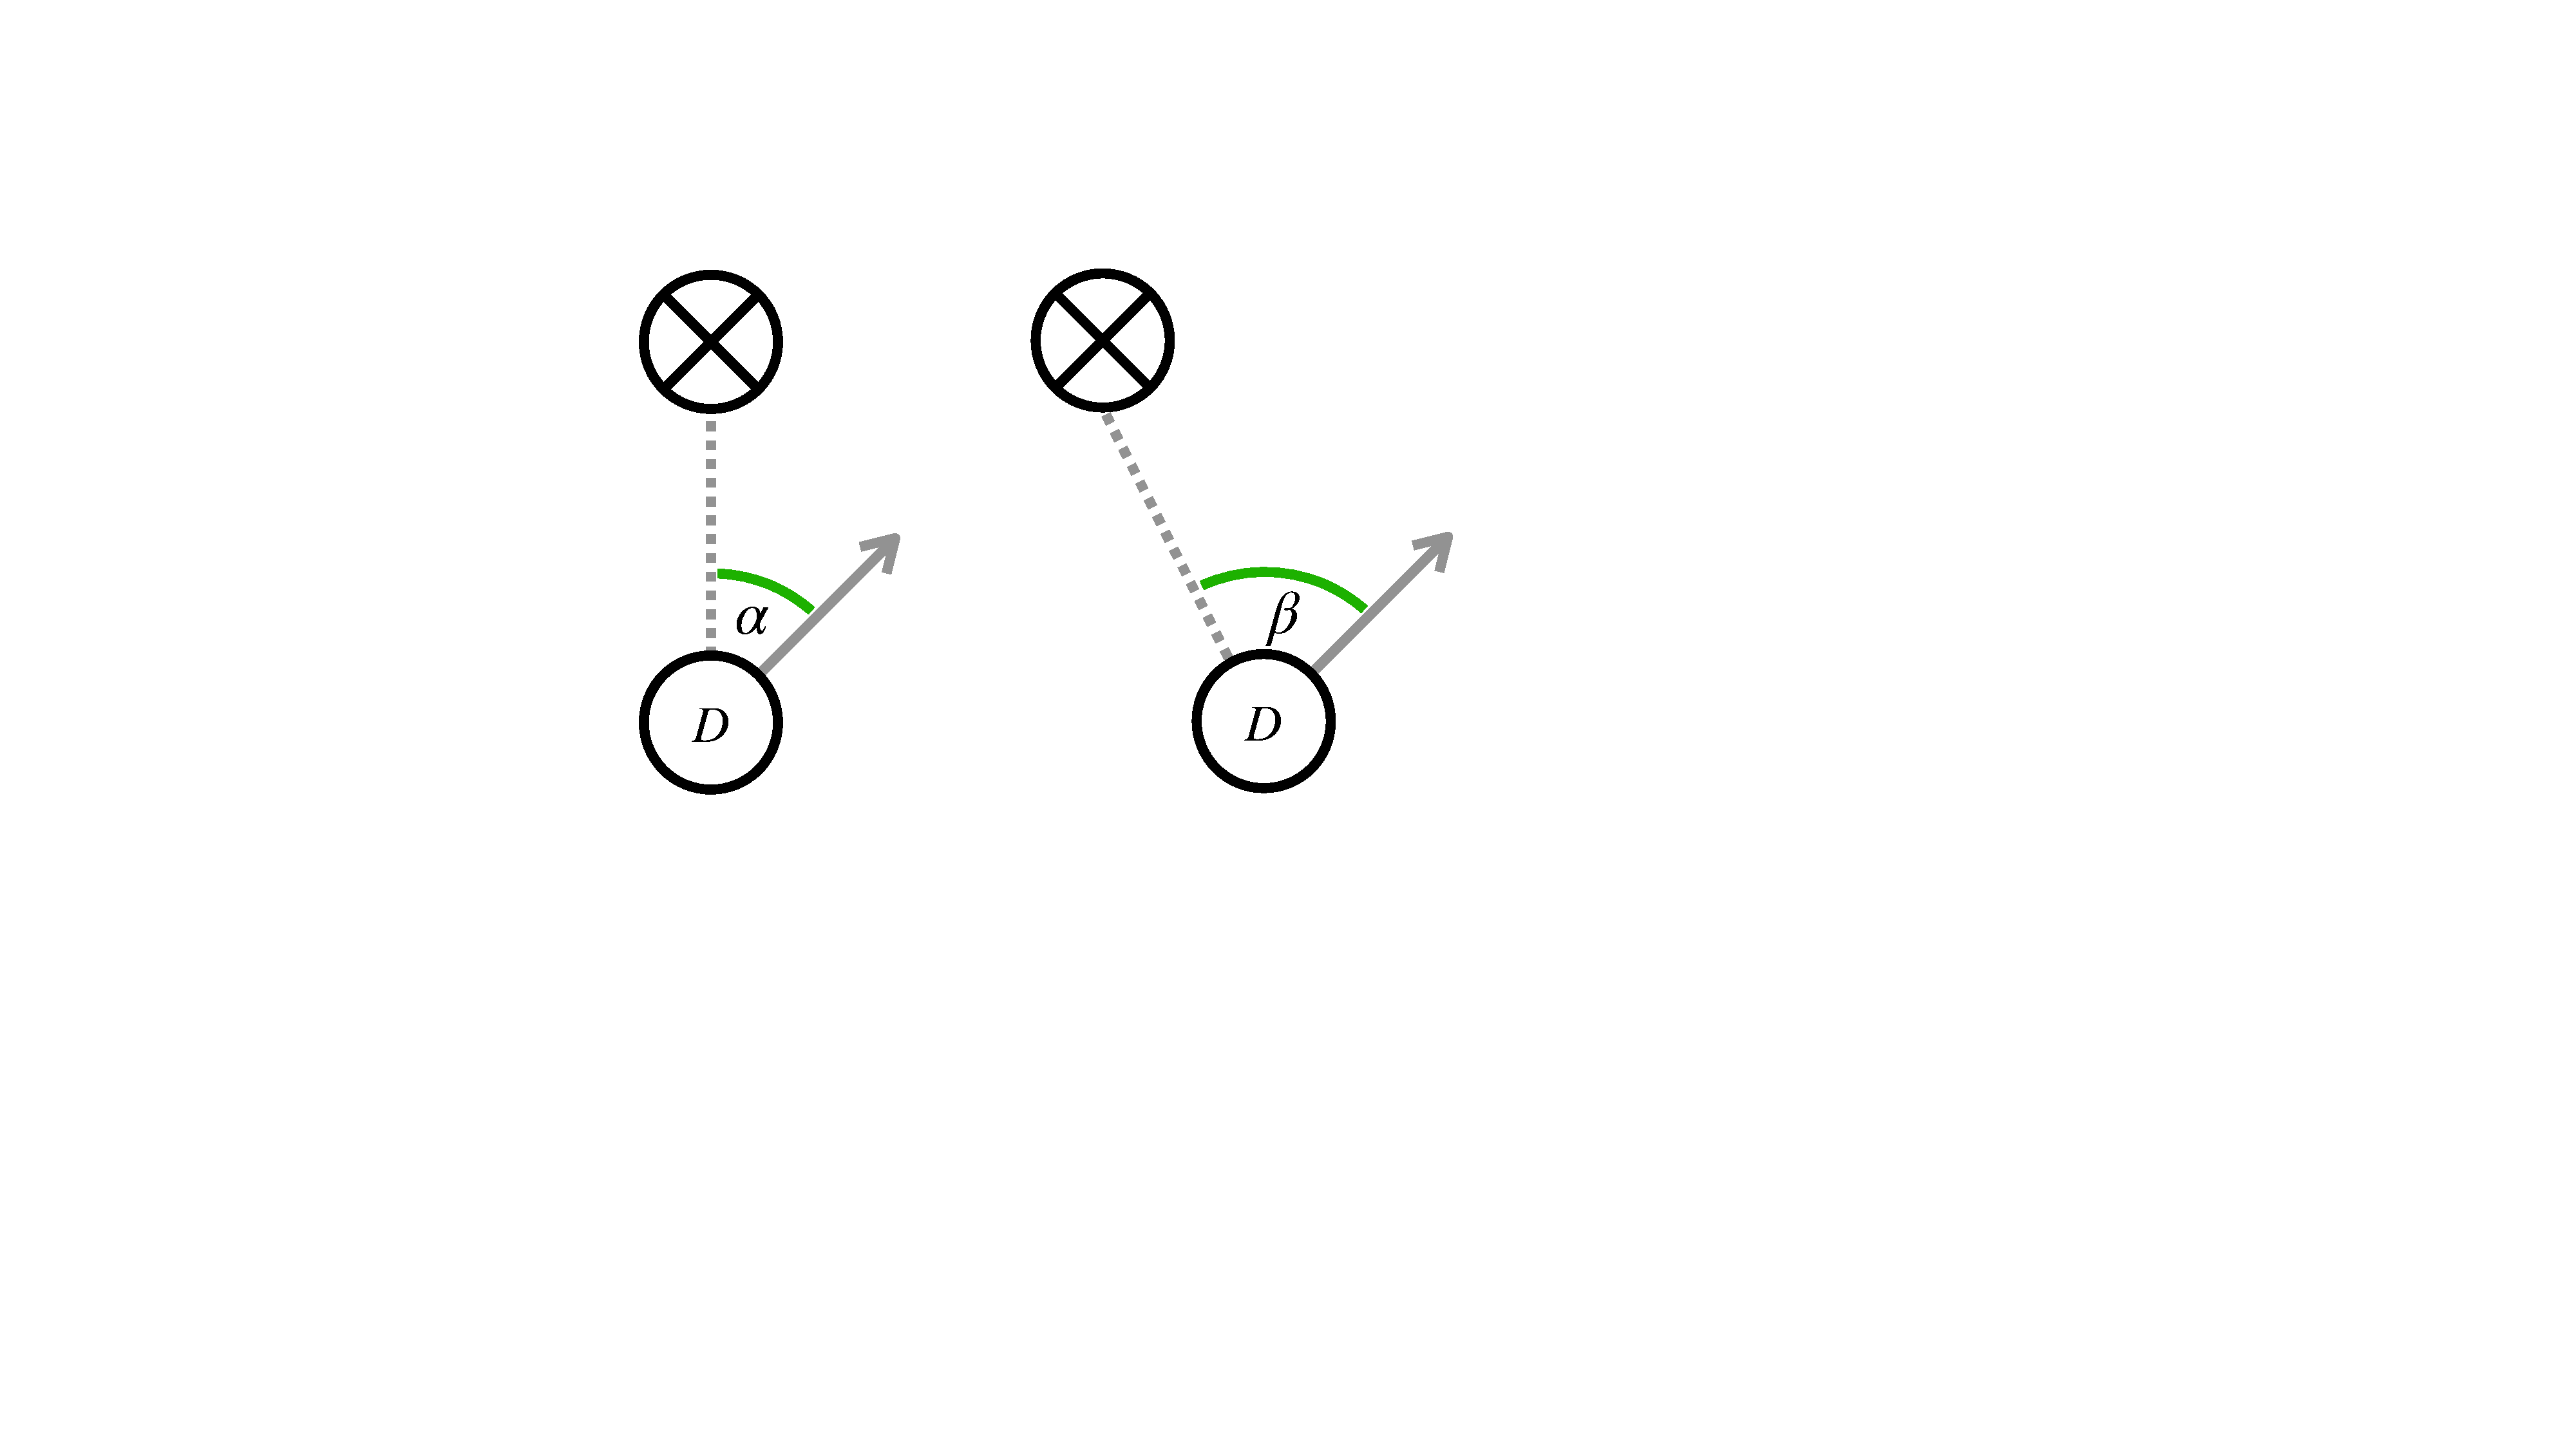
\includegraphics[width=0.5\textwidth]{../assets/dezibot_signal_moving_problem.pdf}
    \caption{Verändernder Beacon"=Winkel $\alpha$ bzw. $\beta$ bei Bewegung des Dezibots ohne Rotation.}
    \label{fig:dezibot_signal_moving_problem}
\end{figure}

Dabei ist dargestellt, wie sich der Beacon"=Winkel $\alpha$ zu $\beta$ verändert, wenn der Dezibot die Position ändert, sich allerdings nicht rotiert, d.h. immer noch in die gleiche Richtung ausgerichtet ist. Dieser Fehler ist nicht trivial lösbar. Hierfür wäre eine Art Selbstortung des Dezibots notwendig, beispielsweise durch eine Triangulation mit einem zweiten Beacon. Dabei müssten die beiden Beacon unterschiedliche Frequenzen aussenden, damit sie unterscheidbar sind (vgl. erwähnter Ansatz oben).

Eine Selbstortung wäre durch mindestens drei weitere Beacon"=Dezibots denkbar, welche jeweils ein WLAN"=Signal aussenden. Durch die Messung der jeweiligen \emph{Wi-Fi Round Trip Time} (Wi-Fi RTT) wäre eine Triangulation der Position auf dem Schachbrett möglich. Ein ähnlicher Implementierungsansatz ist beispielhaft unter~\cite{espressifsystemsshanghaico.ltdFTMExample2024} einsehbar. Diese Methode setzt jedoch eine sehr genaue Zeitmessung (im Nanosekundenbereich) voraus, welche mit dem Dezibot nicht gegeben ist. Folglich stellt sich die Frage, ob diese Methode die notwendige Präzision erreichen kann.

% Zusammenfassung

Zusammenfassend unterscheiden sich die genannten Ansätze in ihrer Komplexität. In der begrenzten Projektzeit war es nicht möglich, diese weiter zu verfolgen, weshalb sie Forschungsgegenstand zukünftiger Projekte sein könnten.


\subsubsection{Verbesserungsansätze}
\label{sec:ir-rotation-improvements}

In diesem Abschnitt werden weitere Versuche zur Verbesserung der Winkelmessung erläutert. Dabei handelt es sich einerseits um den Versuch, die Trigonometrie entsprechend der Winkel der Sensoren anzupassen. Andererseits wurden verschiedene Künstliche Neuronale Netze (\emph{Multi"=Layered"=Perceptron}, MLP) trainiert.

% Trigonometrie

Als erstes wurde versucht, die Trigonometrie, mit der die Winkel aus den Infrarot"=Sensordaten bestimmt werden, anzupassen. Somit sollte das Problem der Sensorplatzierung der Nord"= sowie Süd"=Sensoren entgegengewirkt werden. Daher wurde ein Vorfaktor für die Nord"= und Südwerte bestimmt, welche die Vektoren der Messung in die Richtung der Sensoren ausrichtet. Hintergründe dazu können \autoref{sec:angle-determination-adjustment} kurz nachgelesen werden.

Insgesamt ist dieser Versuch allerdings gescheitert, da die Sensoren zwar nicht auf der $y$-Achse platziert sind. Jedoch sind die dennoch in die korrekte Richtung, d.h. Norden bzw. Süden, ausgerichtet. Somit sind die angepassten Werte, v.a. in Süd"=Richtung, um bis zu 30° abgewichen.

Aus diesem Ergebnis konnte jedoch die Erkenntnis gezogen werden, dass vermutlich nicht die Platzierung der Sensoren, sondern vielmehr die Beine des Dezibots das wahre Problem darstellen, da diese das Sichtfeld der Sensoren beinschränken. Dies ist ein weiteres Problem, dessen Lösung in zukünftigen Arbeiten betrachtet werden kann.

% MLP Regressor

Im Weiteren wurde versucht, ein MLP zu trainieren. Die Eingangsdaten basieren auf den Messungen aus \autoref{sec:measurements-dezibot-angle}, wobei die normalisierten Sensordaten als Feature $\mathbf{X}$ und die erwarteten Winkel als Label $\mathbf{y}$ verwendet.

\begin{equation*}
    \mathbf{X} = \begin{bmatrix}
        n_{1,\text{norm}} & e_{1,\text{norm}} & s_{1,\text{norm}} & w_{1,\text{norm}} \\
        \vdots & \vdots & \vdots & \vdots \\
        n_{n,\text{norm}} & e_{n,\text{norm}} & s_{n,\text{norm}} & w_{n,\text{norm}}
    \end{bmatrix},
    \quad \mathbf{y} = \begin{bmatrix}
        \alpha_1 \\ \vdots \\ \alpha_n
    \end{bmatrix}
\end{equation*}

Das Training wurde mit der Python"=Library \texttt{scikit-learn}\footnote{\url{https://scikit-learn.org/1.6/}} umgesetzt. Dafür wurde ein \texttt{MLP"-Regressor} als Regressionsmodell ausgewählt. Dieses erlaubt unter anderem das überwachte Lernen von nicht"=-linearen Zusammenhängen, wie sie aus den Daten von \autoref{sec:measurements-dezibot-angle} angedeutet sind. Weiterhin ist es durch die Anzahl von versteckten Schichten (\emph{Hidden Layer}) anpassbar~\cite{scikit-learndevelopers117NeuralNetwork2025}. Diese wurde nach ein paar Experimenten auf $(20,20)$ festgesetzt, d.h. jeweils 20~Neuronen in der ersten und zweiten Schicht mit insgesamt zwei versteckten Schichten. Das entsprechende Jupyter"=Notebook kann ebenfalls auf GitHub\footnote{\url{https://github.com/embedded-chess/misc/blob/main/src/angle_determination_adjustment/mlp.ipynb}} eingesehen werden.

Nach einer zufälligen Aufteilung der Daten in Test"= und Trainingsdaten mit einer Aufteilung von 1:5 wurde das Modell trainiert. Nach verschiedenen Anläufen kamen die in \autoref{fig:cnn-mlp-diff} dargestellten Ergebnisse zustande.

\begin{figure}[h]
    \centering
    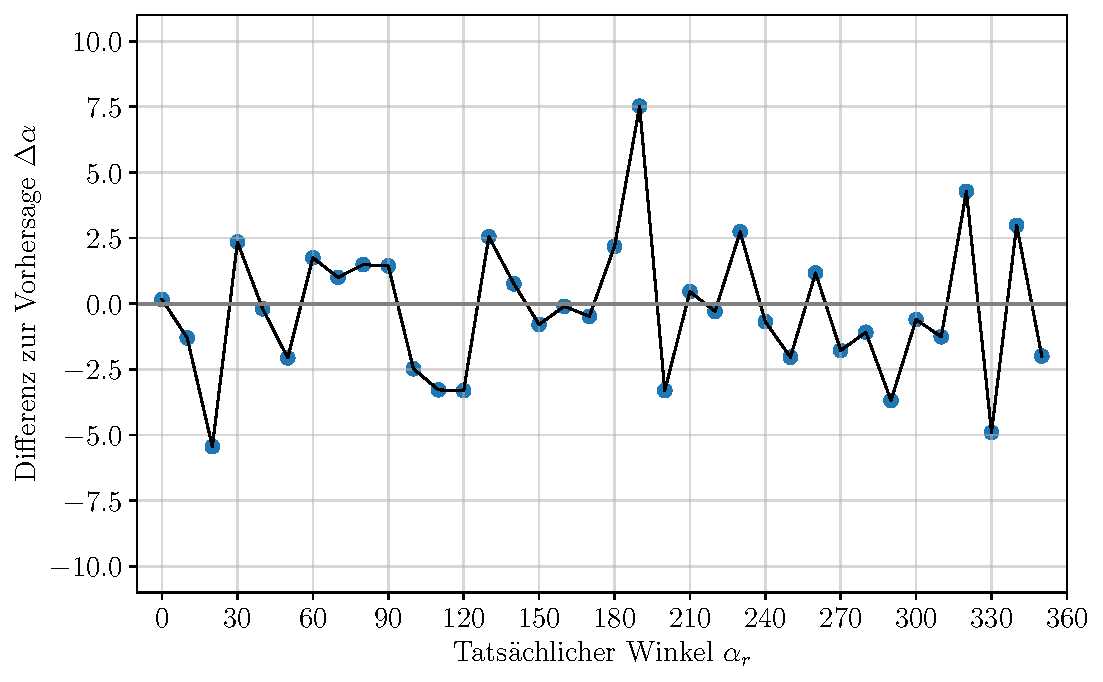
\includegraphics[width=\textwidth]{../plot/angle_adjustment/mlp_sensor_diff.pdf}
    \caption{Diagramm der Differenz $\Delta\alpha$ zwischen vorhergesagten Winkeln vom MLP"=Regressor $\alpha_p$ und dem tatsächlichen Winkel $\alpha_r$ bezüglich des echten Winkels mit $\Delta\alpha = \alpha_p - \alpha_m$.}
    \label{fig:cnn-mlp-diff}
\end{figure}

Vor allem im Vergleich zu \autoref{fig:ir-signal-diff} ist zu erkennen, dass die Differenzen nun statt zwischen ungefähr -10° bis 10° zwischen -7,5° und 7,5° schwanken. Somit ist das Schwankungsintervall kleiner geworden. Da dieser Ansatz allerdings keine ausreichend gute Verbesserung brachte, wurde dieses Modell nicht in das Projekt integriert. Allerdings könnten weiterführende Experimente, bspw. an der Einstellung der Hyperparameter oder Wahl anderer Regressionsmodelle, durchgeführt werden.

Das trainierte Modell wurde gespeichert und kann auf GitHub\footnote{\url{https://github.com/embedded-chess/misc/blob/main/src/angle_determination_adjustment/mlp_regressor_model_sensor_data.onnx}} abgerufen werden. Dieses ist im Standard von \emph{Open Neural Network Exchange} (ONNX)\footnote{\url{https://onnx.ai}} abgespeichert, welches in andere gängige Formate, wie bspw. von TensorFlow (Lite)~\cite{hyodoToolsConvertONNX2025, internationalbusinessmachinescorporationOnnxOnnxtensorflow2022}, umgewandelt werden kann~\cite{scikit-learndevelopersModelPersistence2025}. Somit kann es in Python, aber auch in C++ auf dem Dezibot verwendet werden~\cite{espressifsystemsEspressifEsptflitemicro2025,thetensorflowauthorsTanakamasayukiArduino_TensorFlowLite_ESP322022}, wie bspw. in~\citeauthor{antonovSnskorpion2DezibotLabyrinthSolver2025}~\cite{antonovSnskorpion2DezibotLabyrinthSolver2025}.

Ein weiterer Versuch bestand darin, statt eine MLP"=Regressors eine Support"=Vektor"=Maschine (SVM) als Regressor (\emph{Support Vector Regression}, \texttt{SVR}) zu verwenden. Die Ergebnisse waren jedoch schlechter als die bereits vorhandene Implementierung (vgl. \autoref{sec:angle-determination}), weshalb dieser Ansatz verworfen wurde. 

Ferner wurden die bestimmten Winkel vom Dezibot als Feature und die tatsächlichen Winkel als Label verwendet. Dies ist im oben genannten Jupyter"=Notebook enthalten. Dieser Ansatz führte allerdings zu sehr ähnlichen Schwankungen wie in \autoref{sec:angle-determination}. Eine Ursache könnten die begrenzten Trainingsdaten sein. Insgesamt wurde sich daher entschieden, diesen Ansatz nicht weiter zu verfolgen.


\subsection{Iteration 5: Kalibrierung der Farben}
\label{sec:colour-calibration}

Das Erkennen von Feldern anhand der Farbe ist eng mit der Bewegung verknüpft: Eine Bewegung, wie bspw. die Vorwärtsbewegung um ein Feld, benötigt diese, um ausgeführt zu werden. Allerdings kann die Farberkennung eine Bewegung nur in dem Maße unterstützen, wie letztere selbst zuverlässig funktioniert.

Vorstellbar wäre eine Farberkennung, welche die Mitte eines Feldes exakt erkennt. Somit würde ein Dezibot nur halten, wenn er diese auch erreicht hat. Da die Bewegung jedoch nicht exakt ist, können bereits kleine Abweichung dazu führen, dass ein Dezibot über ein Feld hinausläuft, da er für sich betrachtet nicht exakt in der Mitte steht. Dementsprechend ist es wichtig, für die Farberkennung eine Balance zu finden, welche die Bewegung bestmöglich unterstützt, diese jedoch nicht beeinträchtigt.


\subsubsection{Farbsensor}
\label{sec:colour-calibration-colour-sensor}

Für die Verbesserung der Farberkennung war zunächst der Ansatz, eine Kalibrierung der Farben durchzuführen, um die aktuellen Lichtverhältnisse einzubeziehen. Der Dezibot wird dafür zu Beginn auf ein weißes und ein schwarzes Feld gesetzt, um den Schwellwert anhand der gemessenen Werte anzupassen. Die Kalibrierung wird mit der Funktion \texttt{ECP\-Color\-Detection::""calibrate\-Field\-Color} umgesetzt. In dieser wird jeweils eine Aufforderung auf das Display gedruckt (vgl.~\autoref{fig:colour-calibration-display-print}).

\begin{figure}[h]
\centering
\begin{cminted}{text}
+----------------+    +----------------+
|Calibrate white |    |Calibrate black |
|Please place on |    |Please place on |
|white field     |    |black field     |
|within 2s       |    |within 2s       |
|                |    |                |
|                |    |                |
|                |    |                |
|                |    |                |
+----------------+    +----------------+
\end{cminted}
\caption{Beispiel-Ausgabe für Kalibrierung der Farben.}
\label{fig:colour-calibration-display-print}
\end{figure}

Insgesamt werden an je fünf Positionen auf dem Schachbrett für beide Farben die durchschnittlichen Helligkeitswerte aus jeweils drei Messungen ermittelt. Der Schwellwert für die Farbe weiß wird anhand der niedrigsten Messung und für schwarz anhand der höchsten Messung sowie einem entsprechenden Offset berechnet. Die Implementierung ist in \autoref{code:calibrate-field-color} dargestellt.

\begin{listing}[h]
    \inputminted{cpp}{../assets/code/ECPColorDetection-calibrateFieldColor.cpp}
    \caption{Code"=Ausschnitt zur \texttt{ECP"-Color"-Detection::""calibrate\-Field\-Color}"=Funktion.}
    \label{code:calibrate-field-color}
\end{listing}

Durch die zwei Schwellwerte ergibt sich ein weiterer Zustand, uneindeutig~(\emph{ambiguous}), welcher bei der Bestimmung der aktuellen Feldfarbe auftreten kann. So werden sowohl weiße als auch schwarze Felder erst wahrgenommen, wenn der Dezibot weitestgehend auf jenem Feld steht. Durch den neuen Zustand kann die Funktion \texttt{ECP"-Color"-Detection::""is"-White"-Field} nicht mehr nur einen Wahrheitswert zurückgeben und wurde daher durch \texttt{ECP"-Color"-Detection::""get"-Field"-Color} ersetzt.

Zu Beginn einer Vorwärtsbewegung wird bestimmt, auf welcher Feldfarbe sich der Dezibot befindet. Da \texttt{get\-Field\-Color} jedoch auch \texttt{AMBIGUOUS} zurückgeben kann, muss eine weiter Funktion implementiert werden, welche die wahrscheinlichste Farbe zurückgibt. Dies wird durch \texttt{ECP\-Color\-Detection::""get\-Likely\-Field\-Color} umgesetzt, welche die Farbe zurückgibt, für die die gemessene Helligkeit näher am entsprechenden Schwellwert liegt.

Das Problem, dass der Dezibot eine Farbe erkennt, obwohl er sich nicht vollständig auf dem Feld befindet, wurde experimentell durch die Einführung von zwei zusätzlichen Zuständen behandelt. Dabei wurde neben der Helligkeit, wenn der Dezibot vollständig auf dem Feld steht, auch der hellste bzw. dunkelste Wert gemessen, während der Farbsensor in der Mitte des Feldes positioniert ist. Die Idee war, dass zunächst der Schwellwert für diesen Zustand erreicht werden muss, bevor die tatsächliche Feldfarbe angenommen wird.

Dafür wurde \texttt{Field\-Color} um \texttt{AMBIGUOUS\_BLACK\_TO\_WHITE}~(ABW) sowie \texttt{AMBIGUOUS\_WHITE\_TO\_BLACK}~(AWB) erweitert. Durch diese Zustände ist auch für die Vorwärtsbewegung eine Plausibilitätsprüfung umsetzbar. Wenn nach Erreichen der Übergangszustände ABW und AWB ein anderer Zustand als \texttt{WHITE\_FIELD} oder \texttt{BLACK\_FIELD} erreicht wird, ist der Dezibot wahrscheinlich wieder vom Feld heruntergelaufen. Der Unterschied zwischen der Mitte eines Feldes und einem Punkt weiter außen ist jedoch meistens zu gering, weshalb der Ansatz nicht leistungsfähig ist. 

Dennoch wurde eine Plausibilitätsprüfung für Vorwärtsbewegungen um je ein Feld eingeführt, welche die Anzahl der Bewegungen beschränkt. Wenn also innerhalb von zehn Versuchen die gesuchte Feldfarbe nicht erreicht wurde, ist der Dezibot wahrscheinlich über das Feld hinaus und nicht gerade gelaufen.

Auch das Licht zur Ausbesserung schlechter Lichtverhältnisse wurde in dieser Iteration angepasst. Da dieses nur für die Messungen relevant ist, wird die Verwendung über die Flag \texttt{ECP\-Color"-Detection::""turn\-On\-Color\-Correction\-Light} geregelt. Wenn diese Flag auf \texttt{true} gesetzt ist, wird die LED vor der Helligkeitsmessung mit einer Verzögerung eingeschaltet, um eine präzise Messung zu gewährleisten, und anschließend wieder ausgeschaltet. Auf diese Weise ist erkenntlich, wann die Farbe gemessen wird, und spart somit Energie. Ebenso besteht keine Notwendigkeit außerhalb der \texttt{ECP"-Color"-Detection}"=Klasse mit dem Licht zu interagieren.


\subsubsection{Infrarot"=Farberkennung}
\label{sec:colour-calibration-ir}

Alternativ zur Verwendung des Farbsensors wurde der Idee nachgegangen, die Farbe eines Feldes mithilfe von Infrarot zu bestimmen. Schwarze Felder absorbieren Infrarot"=Licht, während weiße Felder es reflektieren. Anhand der Infrarot"=Sensoren kann überprüft werden, wie viel des ausgesendeten Lichts reflektiert wird. Dafür wird die Infrarot"=LED, welche zentral auf der Unterseite platziert ist, verwendet. Aufgrund der Position dieser kann nach den durchgeführten Experimenten das Verhältnis von schwarzem zu weißem Untergrund bestimmt und somit die Mitte eines Feldes bestimmt werden.

Die Farberkennung verläuft ähnlich zum Ansatz mittels Farbsensor (vgl.~\autoref{sec:colour-calibration-colour-sensor}). Zunächst wird für die Berechnung der Schwellwerte eine Kalibrierung durchgeführt. Die Implementierung is in \autoref{code:calibrate-ir-field-color} dargestellt.Die Schwellwerte berechnen sich mit einem Offset aus 20\% der Differenz. 

\begin{listing}[h]
    \inputminted{cpp}{../assets/code/ECPColorDetection-calibrateIRFieldColor.cpp}
    \caption{Code"=Ausschnitt zur \texttt{ECP"-Color"-Detection::""calibrate\-IR\-Field\-Color}"=Funktion.}
    \label{code:calibrate-ir-field-color}
\end{listing}

Vor der Messung wird die LED mit anschließender Verzögerung in der Funktion \texttt{ECP\-Signal\-Detection::""cumulate\-Infrared\-Values} angeschaltet. Ohne die Verzögerung kann es passieren, dass die LED noch nicht leuchtet. Für die Bestimmung der Feldfarbe sind die einzelnen Infrarot"=Werte nicht relevant, weshalb diese addiert werden. Somit kann die aktuelle Feldfarbe anhand der Summe in der Funktion \texttt{ECP\-Color\-Detection::""measure\-Infrared\-Field\-Color} bestimmt werden. Anschließend wird die LED (ebenfalls mit einer Verzögerung) abgeschaltet, damit sichergestellt ist, dass die LED tatsächlich aus ist. \autoref{code:cumulate-ir-values} zeigt die verkürzte Implementierung. Auch wird mit \texttt{ECP\-Color\-Detection::""calculate\-Likely\-Infrared\-Field\-Color} bestimmt, welcher Schwellwert näher an der aktuellen Farbe liegt.

\begin{listing}[h]
    \inputminted{cpp}{../assets/code/ECPSignalDetection-cumulateInfraredValues.cpp}
    \caption{Verkürzter Code"=Ausschnitt zur \texttt{ECP\-Signal\-Detection::""cumulate\-Infrared\-Values}"=Funktion.}
    \label{code:cumulate-ir-values}
\end{listing}

Die Verzögerungen bei der Verwendung der Infrarot"=LED stammt aus der Implementierung in der \texttt{dezibot}"=Library, in der festgelegt ist, dass diese für eine bestimmte Zeit leuchtet und nicht spontan ausgeschaltet werden kann. Die Verzögerung sorgt dafür, dass für die nachfolgenden Befehle der erwartete Zustand der Infrarot"=LED auch tatsächlich angenommen wurde.

Zur Klasse \texttt{ECP\-Color\-Detection} wurde im Rahmen dieser Iteration die Flag \texttt{use"-Infrared"-Color"-Detection} hinzugefügt, welche bestimmt, ob der Ansatz mittels Infrarot (\texttt{true}) oder RGB (\texttt{false}) zur Erkennung der Feldfarbe verwendet werden soll. Dies kann mittels \texttt{ECP\-Color\-Detection::""set\-Use\-Infrared\-Color\-Detection} verändert werden. Die Funktionen zur Bestimmung der Feldfarbe verändern sich nach außen nicht, wodurch sich die Verwendung in \texttt{ECP\-Movement} ebenfalls nicht verändert.

Beeinträchtigt wird die Farberkennung durch das Beacon, welches ebenfalls Infrarot aussendet und dafür sorgt, dass schwarze Felder als uneindeutig oder sogar als weißes Feld wahrgenommen werden. Um dem entgegen zu wirken, muss das Infrarot"=Licht des Beacons daher während des Messens abgeschaltet werden. Dies könnte bspw. über eine drahtlose Verbindung kommuniziert werden. Da drahtlose Verbindungen jedoch von diesem Projekt ausgeschlossen sind, wurde experimentell dem Ansatz nachgegangen, den Beacon durch periodisches Messen auf andere Infrarot"=Signale reagieren zu lassen.

Dabei wird der nördliche Infrarot"=Sensor des Beacons verwendet, um andere Signale zu messen. Wenn eine bestimmte Stärke erfasst wird, schaltet der Beacon sein Licht aus; sobald kein anderes Infrarot"=Signal wahrgenommen wird, schaltet er es wieder an. Das An- und Ausschalten der LED ist nicht sofort möglich, weshalb auch hier Verzögerungen eingebaut werden mussten, um sicherzustellen, dass die LED den gewollten Status annimmt.

Bei diesem Ansatz ist problematisch, dass das Beacon sein eigenes Infrarot"=Signal wahrnimmt, trotz der Verdeckung durch das vordere Bein, wie es in \autoref{fig:dezibot-bottom} dargestellt ist. Dies führt dazu, dass der Beacon periodisch seine LED an- und wieder ausstellt. So kann es durch die Perioden dazu führen, dass die Rotation länger dauert, da der Dezibot ggf. warten muss, bis er wieder ein Infrarot"=Signal wahrnimmt. Der Ansatz funktioniert demnach trotzdem, wenn ausreichend lange vor einer Infrarot"=Farbmessung verzögert wird. So hat das Beacon Zeit in einer Phase, in der sein eigenes Licht aus ist, das Infrarot"=Licht vom Dezibot wahrzunehmen. Dies funktioniert jedoch nicht immer, da aus den Experimenten hervorgeht, dass bei einer Distanz, in der das Beacon das Licht für die Farbmessung nicht erfasst, die Messung beeinträchtigt werden kann. Dieser experimentelle Ansatz für das Beacon wurde im Programm \texttt{ir\_emitter\_ir\_color\_detection.ino} sowie in einem Video\footnote{\url{https://github.com/embedded-chess/doc/raw/refs/heads/main/assets/videos/beacon_turns_off_when_dezibot_measures_ir.mp4}} festgehalten. In dem Video wird der Fall dargestellt, bei dem das Beacon (links im Bild) in der Aus"-Phase das Infrarot"=Licht vom Dezibot wahrnimmt. So tritt nie der Fall ein, dass zu dem Zeitpunkt, wo der Dezibot die Werte misst -- kurz vor dem Ausschalten des Infrarot"=Lichts -- das Beacon Infrarot"=Licht ausstrahlt.

% Ansatz: manuelle Nutzerintervention

Aufgrund der Unzuverlässigkeit des An- und Ausschaltens der Infrarot"=LEDs sowie Problemen ab einer bestimmten Distanz, wurde ein weiterer Ansatz implementiert. Dieser besteht darin, vor der eigentlichen Messung, störende Infrarot"=Signale zu erkennen. Falls solche gemessen werden, wird eine Ausgabe auf das Display gedruckt, welche dazu auffordert, diese zu entfernen. Diese ist in \autoref{fig:display-interfering-ir} dargestellt.

\begin{figure}[h]
\centering
\begin{cminted}{text}
+----------------+
|Interfering IR  |
|signal!         |
|Trying again... |
|                |
|                |
|                |
|                |
|                |
+----------------+
\end{cminted}
\caption{Aufforderung zur Entfernung störender Infra\-rot-Signal\-quellen vor Infrarot"=Farbmessung}
\label{fig:display-interfering-ir}
\end{figure}

Die Ausgabe bleibt, analog zu \autoref{sec:angle-determination}, so lange bestehen, bis keine störende Signale mehr messbar sind, um die Farbmessung nicht zu verfälschen.

Innerhalb des Rahmens unseres Projektes konnte somit eine zufriedenstellende Zwischenlösung gefunden werden. Der manuelle Eingriff kann in Zukunft durch eine drahtlose Verbindung ersetzt werden.
